%%%%%%%%%%%%%%%%%%%%%%%%%%%%%%%%%%%%%%%%%%%%%%%%%%%%%%%%%%%%%%%%%%%%%
%% This is a (brief) model paper using the achemso class
%% The document class accepts keyval options, which should include
%% the target journal and optionally the manuscript type. 
%%%%%%%%%%%%%%%%%%%%%%%%%%%%%%%%%%%%%%%%%%%%%%%%%%%%%%%%%%%%%%%%%%%%%
\documentclass[journal=jacsat,manuscript=article]{achemso}
\usepackage{multicol}
\usepackage{graphicx}% Include figure files
\usepackage{graphicx}% Include figure files
\usepackage{dcolumn}% Align table columns on decimal point
\usepackage{bm}% bold math
%\usepackage[mathlines]{lineno}% Enable numbering of text and display math
%\linenumbers\relax % Commence numbering lines
\usepackage{pgffor}
\usepackage[utf8]{inputenc}
\usepackage[T1]{fontenc}
\usepackage{mathptmx}
\usepackage{listings}
\lstset{language=Python}
\usepackage{rotating} % Rotating table
\usepackage{caption}
\usepackage{subcaption}

\usepackage{color}
\usepackage{dcolumn} % decimal align in tables
\usepackage{bm} % bold math
\usepackage{graphicx}
\usepackage{multirow} % for table cells to span rows
\usepackage{pifont} % for checkmarks
\usepackage{epsfig}
\usepackage{amsmath} % matrix
% \usepackage{subfigure}
\usepackage{float}
\usepackage{booktabs}
\usepackage{tabularx}
\usepackage{natbib}
\usepackage{gensymb}
\setlength{\paperwidth}{8.5in}
\setlength{\paperheight}{11.0in}
\usepackage{rotating}
\usepackage{threeparttable}
\usepackage{comment}
%for corrections
\usepackage[normalem]{ulem}
% \usepackage{xr-hyper}
\usepackage[hidelinks]{hyperref} % allows hyperlinking for references
%%%%%%%%%%%%%%%%%%%%%%%%%%%%%%%%%%%%%%%%%%%%%%%%%%%%%%%%%%%%%%%%%%%%%
%% Place any additional packages needed here.  Only include packages
%% which are essential, to avoid problems later. Do NOT use any
%% packages which require e-TeX (for example etoolbox): the e-TeX
%% extensions are not currently available on the ACS conversion
%% servers.
%%%%%%%%%%%%%%%%%%%%%%%%%%%%%%%%%%%%%%%%%%%%%%%%%%%%%%%%%%%%%%%%%%%%%
\usepackage[version=3]{mhchem} % Formula subscripts using \ce{}
\usepackage{xcolor}
% \usepackage{xr-hyper}
\usepackage{xr-hyper}
\usepackage{xr}


\usepackage[hidelinks]{hyperref} % allows hyperlinking for references

% \usepackage{hyperref}
\usepackage{amsmath,amssymb,amsthm}
\usepackage{mathtools,physics}


\usepackage{subcaption}
\usepackage{caption}
% \usepackage{titling}
%%%%%%%%%%%%%%%%%%%%%%%%%%%%%%%%%%%%%%%%%%%%%%%%%%%%%%%%%%%%%%%%%%%%%
%% If issues arise when submitting your manuscript, you may want to
%% un-comment the next line.  This provides information on the
%% version of every file you have used.
%%%%%%%%%%%%%%%%%%%%%%%%%%%%%%%%%%%%%%%%%%%%%%%%%%%%%%%%%%%%%%%%%%%%%
%%\listfiles

%%%%%%%%%%%%%%%%%%%%%%%%%%%%%%%%%%%%%%%%%%%%%%%%%%%%%%%%%%%%%%%%%%%%%
%% Place any additional macros here.  Please use \newcommand* where
%% possible, and avoid layout-changing macros (which are not used
%% when typesetting).
%%%%%%%%%%%%%%%%%%%%%%%%%%%%%%%%%%%%%%%%%%%%%%%%%%%%%%%%%%%%%%%%%%%%%
\newtheorem{theorem}{Theorem}[section]
\newtheorem{corollary}{Corollary}
\newtheorem{lemma}[theorem]{Lemma}
\newtheorem{proposition}{Proposition}
\newtheorem{conjecture}{Conjecture}
\newtheorem{definition}[theorem]{Definition}
\newtheorem{assumption}[theorem]{Assumption}
% \newtheorem{example}[theorem]{Example}
\newtheorem{example}{Example}[section]
\newtheorem{remark}{Remark}

% Add line numbers, as requested by Nature
\usepackage{lineno}
% \linenumbers


\newcommand*\mycommand[1]{\texttt{\emph{#1}}}
\newcommand{\noteg}[1]{\textcolor{red}{({Grier: #1})}}
\newcommand{\notek}[1]{\textcolor{darkspringgreen}{({Kostas: #1})}}


%%%% HELPER CODE FOR DEALING WITH EXTERNAL REFERENCES
% (from an answer by cyberSingularity at http://tex.stackexchange.com/a/69832/226)
%%%

\usepackage{xcite}

%%%%%%%%%%%%%%%%%%%%%%%%%%%%%%%%%%%%%%%%%%%%%%%%%%%%%%%%%%%%%%%%%%%%%%%%
%----Helper code for dealing with external references----
% (by cyberSingularity at http://tex.stackexchange.com/a/69832/226)

\usepackage{xr}
\makeatletter

\newcommand*{\addFileDependency}[1]{% argument=file name and extension
\typeout{(#1)}% latexmk will find this if $recorder=0
% however, in that case, it will ignore #1 if it is a .aux or 
% .pdf file etc and it exists! If it doesn't exist, it will appear 
% in the list of dependents regardless)
%
% Write the following if you want it to appear in \listfiles 
% --- although not really necessary and latexmk doesn't use this
%
\@addtofilelist{#1}
%
% latexmk will find this message if #1 doesn't exist (yet)
\IfFileExists{#1}{}{\typeout{No file #1.}}
}\makeatother

\newcommand*{\myexternaldocument}[1]{%
\externaldocument{#1}%
\addFileDependency{#1.tex}%
\addFileDependency{#1.aux}%
}
%------------End of helper code--------------

% put all the external documents here!
\myexternaldocument{SI}
\newcommand{\siref}[1]{\ref{#1}}
%%%%%%%%%%%%%%%%%%%%%%%%%%%%%%%%%%%%%%%%%%%%%%%%%%%%%%%%%%%%%%%%%%%%%%%%


%%%%%%%%%%%%%%%%%%%%%%%%%%%%%%%%%%%%%%%%%%%%%%%%%%%%%%%%%%%%%%%%%%%%%
%% The document title should be given as usual. Some journals require
%% a running title from the author: this should be supplied as an
%% optional argument to \title.
%%%%%%%%%%%%%%%%%%%%%%%%%%%%%%%%%%%%%%%%%%%%%%%%%%%%%%%%%%%%%%%%%%%%%
\title{A Combinatorial Search of Parameterized Quantum Circuit Learning for Chemical Applications}
%%%%%%%%%%%%%%%%%%%%%%%%%%%%%%%%%%%%%%%%%%%%%%%%%%%%%%%%%%%%%%%%%%%%%
%% Meta-data block
%% ---------------
%% Each author should be given as a separate \author command.
%%
%% Corresponding authors should have an e-mail given after the author
%% name as an \email command. Phone and fax numbers can be given
%% using \phone and \fax, respectively; this information is optional.
%%
%% The affiliation of authors is given after the authors; each
%% \affiliation command applies to all preceding authors not already
%% assigned an affiliation.
%%
%% The affiliation takes an option argument for the short name.  This
%% will typically be something like "University of Somewhere".
%%
%% The \altaffiliation macro should be used for new address, etc.
%% On the other hand, \alsoaffiliation is used on a per author basis
%% when authors are associated with multiple institutions.
%%%%%%%%%%%%%%%%%%%%%%%%%%%%%%%%%%%%%%%%%%%%%%%%%%%%%%%%%%%%%%%%%%%%%
\author{Grier M. Jones}
\affiliation[UTSG ECE]{
The Edward S. Rogers Sr. Department of Electrical and Computer Engineering, 
University of Toronto, 
10 Kings College Road, Toronto, Ontario, 
Canada M5S 3G4}
\alsoaffiliation[UTM CHEM]{
Department of Chemical and Physical Sciences, 
University of Toronto Mississauga, 
3359 Mississauga Road, Mississauga, Ontario, 
Canada L5L 1C6}

\author{Nick Taylor}
\affiliation[UTSG ECE]{
The Edward S. Rogers Sr. Department of Electrical and Computer Engineering, 
University of Toronto, 
10 Kings College Road, Toronto, Ontario, 
Canada M5S 3G4}
          
\author{Viki Kumar Prasad}
\affiliation[UTSG ECE]{
The Edward S. Rogers Sr. Department of Electrical and Computer Engineering, 
University of Toronto, 
10 Kings College Road, Toronto, Ontario, 
Canada M5S 3G4}
\alsoaffiliation[UTM CHEM]{
Department of Chemical and Physical Sciences, 
University of Toronto Mississauga, 
3359 Mississauga Road, Mississauga, Ontario, 
Canada L5L 1C6}



\author{Ulrich Fekl}
\affiliation[UTM CHEM]{
Department of Chemical and Physical Sciences, 
University of Toronto Mississauga, 
3359 Mississauga Road, Mississauga, Ontario, 
Canada L5L 1C6}
\email{ulrich.fekl@utoronto.ca}

\author{Hans-Arno Jacobsen}
\affiliation[UTSG ECE]{
The Edward S. Rogers Sr. Department of Electrical and Computer Engineering, 
University of Toronto, 
10 Kings College Road, Toronto, Ontario, 
Canada M5S 3G4}
\email{jacobsen@eecg.toronto.edu}
%%%%%%%%%%%%%%%%%%%%%%%%%%%%%%%%%%%%%%%%%%%%%%%%%%%%%%%%%%%%%%%%%%%%%
%% Some journals require a list of abbreviations or keywords to be
%% supplied. These should be set up here, and will be printed after
%% the title and author information, if needed.
%%%%%%%%%%%%%%%%%%%%%%%%%%%%%%%%%%%%%%%%%%%%%%%%%%%%%%%%%%%%%%%%%%%%%
\abbreviations{}
\keywords{American Chemical Society, \LaTeX}

%%%%%%%%%%%%%%%%%%%%%%%%%%%%%%%%%%%%%%%%%%%%%%%%%%%%%%%%%%%%%%%%%%%%%
%% The manuscript does not need to include \maketitle, which is
%% executed automatically.
%%%%%%%%%%%%%%%%%%%%%%%%%%%%%%%%%%%%%%%%%%%%%%%%%%%%%%%%%%%%%%%%%%%%%
\newcommand{\R}{\mathbb{R}}

\begin{document}

\section{Abstract}
The rapid growth of quantum computing has seen a rise in the development of applicable near-term quantum algorithms. A promising candidate to run on current noisy intermediate-scale quantum (NISQ) hardware is quantum machine learning (QML). Parameterized quantum circuits can be learned as models in a hybrid classical-quantum approach. It has been shown that QML models may need less training data to generalize compared to classical methods. Although QML has been explored largely within classification tasks, regression tasks have received much less attention. Existing studies have only utilized few qubits and lack relevant practical applications. We will discuss our work on the development and comparisons of QML models for highly desired prediction of chemical properties such as bond dissociation energies and barrier height energies. Our work investigates the trainability, expressibility, and generalization capability of various quantum models for the purpose of regression of molecular properties. Our work also provides a benchmark against classical machine learning models and implications of using error mitigation techniques for QML. \par

\newpage
\textcolor{red}{Reorganize}
\begin{itemize}
	\item Abstract
	\item Introduction
	\item Methods
	\item Datasets
	\item Results
	\begin{itemize}
		\item Function fitting 
		\begin{itemize}
			\item Classical testing
			\item All (5 + 16 qubit)
			\item RUD + AL (5 + 16 qubit)
			\item Error mitigation
			\item Real device
		\end{itemize}
		\item DDCC (5 qubit only because classically it can be done with 5 features!)
		\begin{itemize}
			\item Classical testing
			\item Truncated  5 qubit set (based on BSE 5 qubit cost analysis)
			\item RUD + AL (5)
			\item Error mitigation
			\item Real device
		\end{itemize}
		\item BSE
		\begin{itemize}
			\item Classical testing
			\item All 5 qubit
			\item Truncated 16 qubit set (cost analysis 5 qubit)
			\item RUD + AL (5 + 16 qubit)
			\item Error mitigation
			\item Real device
		\end{itemize}				
	\end{itemize}
	\item Discussion and Conclusion
\end{itemize}

\newpage
\section{Introduction}
\cite{prasad_applications_2024}
\cite{suzuki_predicting_2020}
\cite{mitarai_quantum_2018}
\cite{sim_expressibility_2019}
\cite{hatakeyama-sato_quantum_2023}
\cite{krenn_artificial_2023}
\cite{benedetti_parameterized_2019}
\cite{biamonte_quantum_2017}




As current quantum hardware grows, much attention is brought to find applicable uses for the potentially powerful new technology while it continues to grow. Current research in the areas of developing quantum algorithms for use with current noisy intermediate-scale quantum (NISQ) hardware lays the foundation for understanding and applying quantum computing. These near-term algorithms have seen a wide deployment across many areas of science and technology as the field grows. Computational chemistry is a natural such candidate for quantum computing applications due to the quantum nature of many problems in the field. An especially important problem is that of calculating the bond separation energies of (molecules?). Efficient and accurate predictions of these values can aid research in material science and drug discovery.\par

One of the most promising near-term applications of quantum computing within any field has been quantum machine learning (QML). The advantages of QML comes largely from its ability to be readily deployed on quantum computers with few qubits, and its potential to speedup problems with minimal loss of accuracy. The number of qubits needed for a QML model is determined primarily by the number of features in the dataset. As there exist data science techniques developed in the realm of classical machine learning to reduce feature spaces, they can be adopted over to reduce problems to a suitable number of qubits. Further, since QML only needs to train once, it has potential to perform faster when compared to other current NISQ algorithms such as the variational quantum eigensolver, which needs to be trained separately for each problem. \par

Quantum machine learning has been widely applied to classification tasks with much success. However, little research has been done to understand its capabilities for regression. Previous works have set important groundwork to the understanding of QML for regression by theoretically formulating upper bounds for the generalization error. Most notably, this research suggests that with an efficiently implemented QML model can achieve good generalizability with modest training data sizes.  This highlights a potential for QML models to outperform and out-generalize classical models. Further understanding and verification of this, however, requires numerical validation and demonstration, and while some experimental work has been done, it remains limited to few qubits with little practical application.\par 

Our work expands on the current knowledge base by providing a comprehensive exploration of QML for regression. Specfically, we will by applying QML to the problem of calculating bond dissociation enthalpies of various molecules. This demonstrates 
a practical application of regression in QML with many applications. The efficient and accurate prediction of these chemical properties can aid research in material science and drug discovery with far reaching implications. Our work serves to benchmark QML and test its capabilities within this context. \par

\section{Methods}
Quantum machine learning is a hybrid classical-quantum approach utilizing parameterized quantum circuits. Typical hybrid algorithms consist of shallow circuit depth of one qubit rotations and two qubit entangling gates. In the context of machine learning, we can subdivide our circuit into three components: the encoder, the variational circuit, and the act of measuring to estimate predictions. The encoder takes our $n$-dimensional data $\bm x \in \R^n$ and encodes it into a unitary feature map $U(\bm x)$ in our working Hilbert Space. This unitary acts on our initialized state $\ket{0}^{\otimes n'}$ to produce the state $U(\bm x) \ket{0}^{\otimes n'}$. It is usual to take $n' = n$ and for each feature $x_i$ to correspond to a qubit. With $n < n'$, features can be repeated across the qubits present in the system. Further elaboration will be discussed with specific encoding circuits. After the encoder produces the state $U(\bm x)\ket{0}^{\otimes n}$, we then tune the state with a parameterized unitary $U(\bm \theta)$ to transform the state into a meaningful prediction. Finally, some configuration of qubits are measured to produce expectation values $\hat y_k$ for our data labels $y_i$ which we then use to minimize a loss function. An obstacle in creating quantum models is there is no way to determine the best encoding or variational circuit for the problem. As such, this paper explores many different encoding and variational circuits. \par

\subsection{Encoder Circuit}
Representation of the data in any machine learning context is a crucial factor in its success. In a classical sense, this can be thought of as generating features and selecting the appropriate features to input into your model. In the quantum context, however, there is the additional question of how to translate the data into the Hilbert space. Different proposed  methods include angle encoding, and amplitude encoding. Following the work done by Suzuki and Katouda, we explore three base encoders composed together with entangling operations. Additionally, we explore the  IQP encoding as given in PennyLane. \par

We composed circuits out of primary rotation blocks and entangling blocks. These rotation blocks include the one proposed by Mitrai et al.\cite{mitarai_quantum_2018}, a single angle rotation, and a double rotation encoder:
\begin{align}
    U_{A1} &= \prod_{i=1}^n R^Y_i(x_i) \\
    U_{A2} &= \prod_{i=1}^n R^Y_i(x_i) R^Z_i(x_i) \\
    U_{M}  &= \prod_{i=1}^n R^Z_i(\arccos x_i^2) R^Y_i(\arcsin x_i^2)
\end{align}
Where $R^j_i$ is a rotation about the $j$ axis on qubit $i$. It's clear to see that this method of encoding imposes a restriction on the number of features to the number of qubits. With this encoding method, it is possible to use more features than qubits and to re-encode the features along the remaining qubits. Then, to compose these encoders together we use entangling circuits that entangle adjacent qubits using either CNOT or CZ entangling operations. These encoding circuits can be seen presented in Figure \ref{fig: idk circuits or something}. 

\subsection{Variational Circuit}
After encoding the data, we have a quantum circuit in a state $U_{\text{enc}}(\bm x)\ket{0}^{\otimes n}$. We need to act on this state with a unitary that has parameters which can be tuned in our machine learning model. Choosing this circuit ansatz can greatly dictate the performance of a given model. Model performance can be greatly influenced by the variational circuit chosen as well as the depth of the circuit as we will later show. It is not obvious which circuit we should pick for our given problem, especially given that our algorithm is not physically motivated like other popular parameterized quantum circuit algorithms. We have gathered a list of 12 variational circuit blocks from previous works and libraries which we will then benchmark for our particular problem. These circuits each can be decomposed into individual rotation gates and two-qubit entangling gates. \par
After our variational circuit acts on our state we have the state:
\begin{align}
    \ket\psi &= U_{\text{var}}(\bm\theta)U_{\text{enc}}(\bm x)\ket{0}^{\otimes n} \label{eq: psi}
\end{align}
where $\bm \theta$ is our parameter vector to be tuned in learning. We can further modify this state; by repeating variational circuit blocks we create a more rich and complex model with a better ability to explore the Hilbert space. This would give us the state:
\begin{align}
    \ket\psi &= U_{\text{var}}(\bm\phi)U_{\text{var}}(\bm\theta)U_{\text{enc}}(\bm x)\ket{0}^{\otimes n} \label{eq: layers}
\end{align}
However, as we are interested in NISQ applications, it should be noted that increasing layer depths creates decoherence in quantum devices. Additionally, we can use the idea of data re-uploading to create redundancies in the encoding of the model to explore a richer feature space. 
\begin{align}
    \ket\psi &= U_{\text{var}}(\bm\phi)U_{\text{enc}}(\bm x)U_{\text{var}}(\bm\theta)U_{\text{enc}}(\bm x)\ket{0}^{\otimes n} \label{eq: re-up}
\end{align}
This paper uses and compares both the data re-uploading and increased depth approaches of creating more complicated models. 

\subsection{Measurement}
After our system is in state $\ket\psi$ as given by either \eqref{eq: psi}, \eqref{eq: layers} or \eqref{eq: re-up} we can measure our system to generate a predicted value $\hat y_i$. At this point in the algorithm, any loss function can be used. In our simplest system, we measured the first qubit so that,
\begin{align}
    \hat y_i &= \langle Z_0 \rangle _\psi 
\end{align}
for a $\psi$ generated by the $k$th data point. Then, we have the loss function we are trying to minimize as,
\begin{align}
    \mathcal{L}(\bm{\hat y}) &= \sum_i^N \frac{(y_i - \hat y_i)^2}{N}
\end{align}

\subsection{Implementation}
Our work was implemented in Python using PennyLane for constructing the quantum circuits, and Qulacs as a primary backend for simulating the circuits. The optimization was implemented using the scipy.optimize module from the SciPy library. Classical models were implemented using scikit-learn while processing of the data was handled with Pandas, NumPy, and SciPy libraries.  


Simulated using FakeQuebecbackend

\subsection{Dataset}
We trained our models using three datasets: a function fitting dataset, consisting of a noisy linear, quadratic, and sine function, used for model calibration; a dataset consisting of electronic structure features to predict wavefunctions using the data-driven coupled-cluster scheme of Townsend and Vogiatzis \cite{townsend_data-driven_2019}; and a dataset of bond separation energies (BSE) of molecules, where the feature set encodes structural information of each molecule. 

For the function fitting dataset, there is only one feature per target value.
For the DDCC dataset, there are initially X features, reduced down to 5 and 16 features, respectively, using SHapley Additive exPlanation (SHAP) values.\cite{lundberg_unified_2017} 


\begin{equation}
	t^{ab}_{ij(\text{MP2})} = \frac{\mel{ij}{}{ab}}{\varepsilon_{i}+\varepsilon_{j}-\varepsilon_{a}-\varepsilon_{b}}
	\label{eq:MP2_t2}
\end{equation}

For each $t^{ab}_{ij(\text{CCSD})}$, orbital energies ($\varepsilon_{i},\varepsilon_{j},\varepsilon_{a},\varepsilon_{b}$), Coulomb and exchange integrals ($J^{i}_{a},J^{j}_{b},K^{a}_{i},K^{b}_{j}$), binary feature whether two electrons are promoted to the same virtual orbital, the initial MP2 amplitudes, along with the numerator (two-electron integrals ($\mel{ij}{}{ab}$)) and denominator $\varepsilon_{i}+\varepsilon_{j}-\varepsilon_{a}-\varepsilon_{b}$.



For the BSE dataset, various molecular representations are explored, and we settled on using Morgan fingerprints with X parameters. 
For the feature reduction, we use PCA, as explained in Section \ref{subsubsection:BSE}.




% Make distribution plot
%\begin{figure}[H]
%	\centering
%	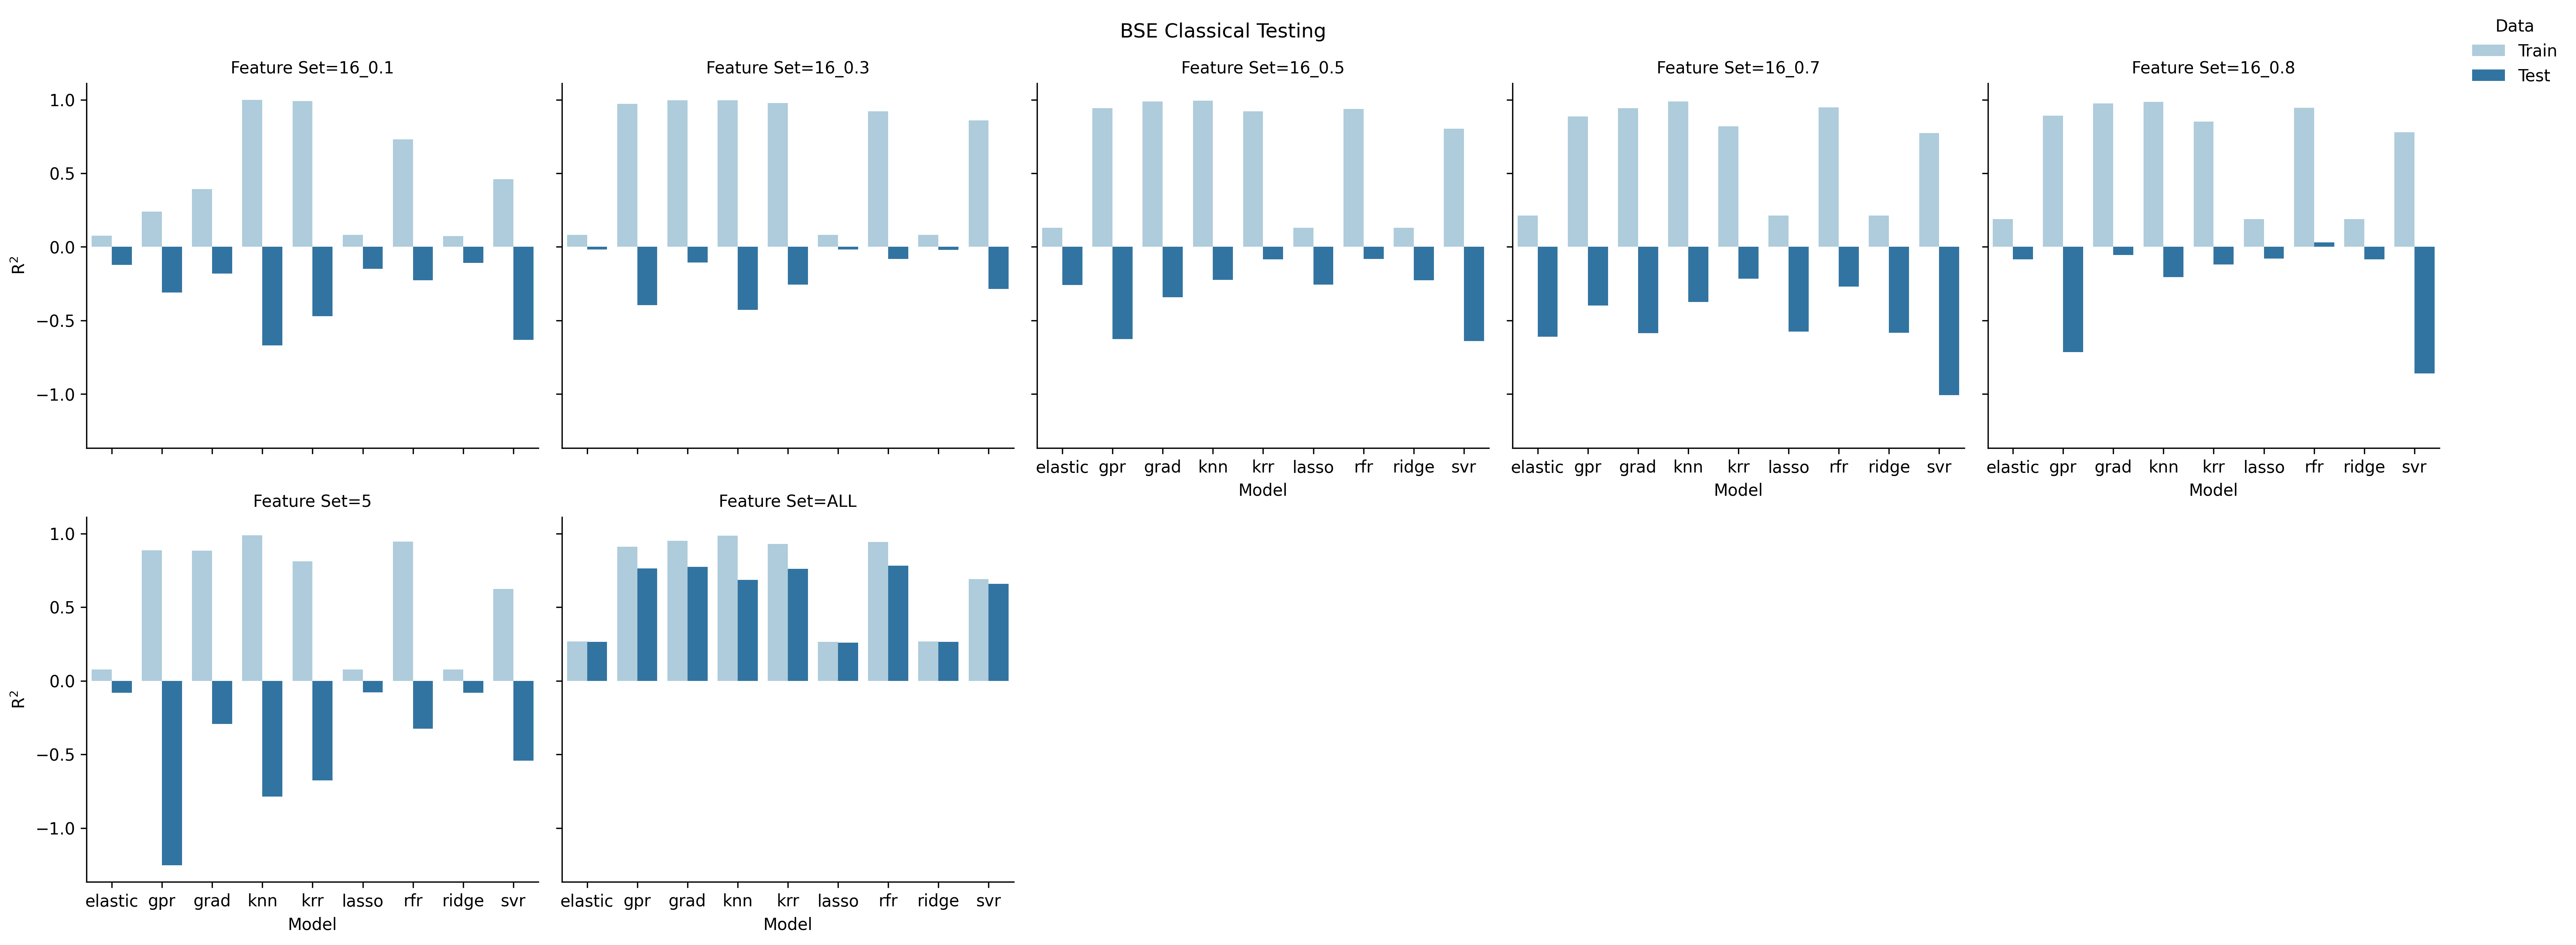
\includegraphics[width=\linewidth]{images/BSE.png}
%	\caption{BSE}
%	\label{fig:BSE}
%\end{figure}


\begin{figure}[H]
	\centering
	\begin{subfigure}[b]{0.3\textwidth}
		\centering
		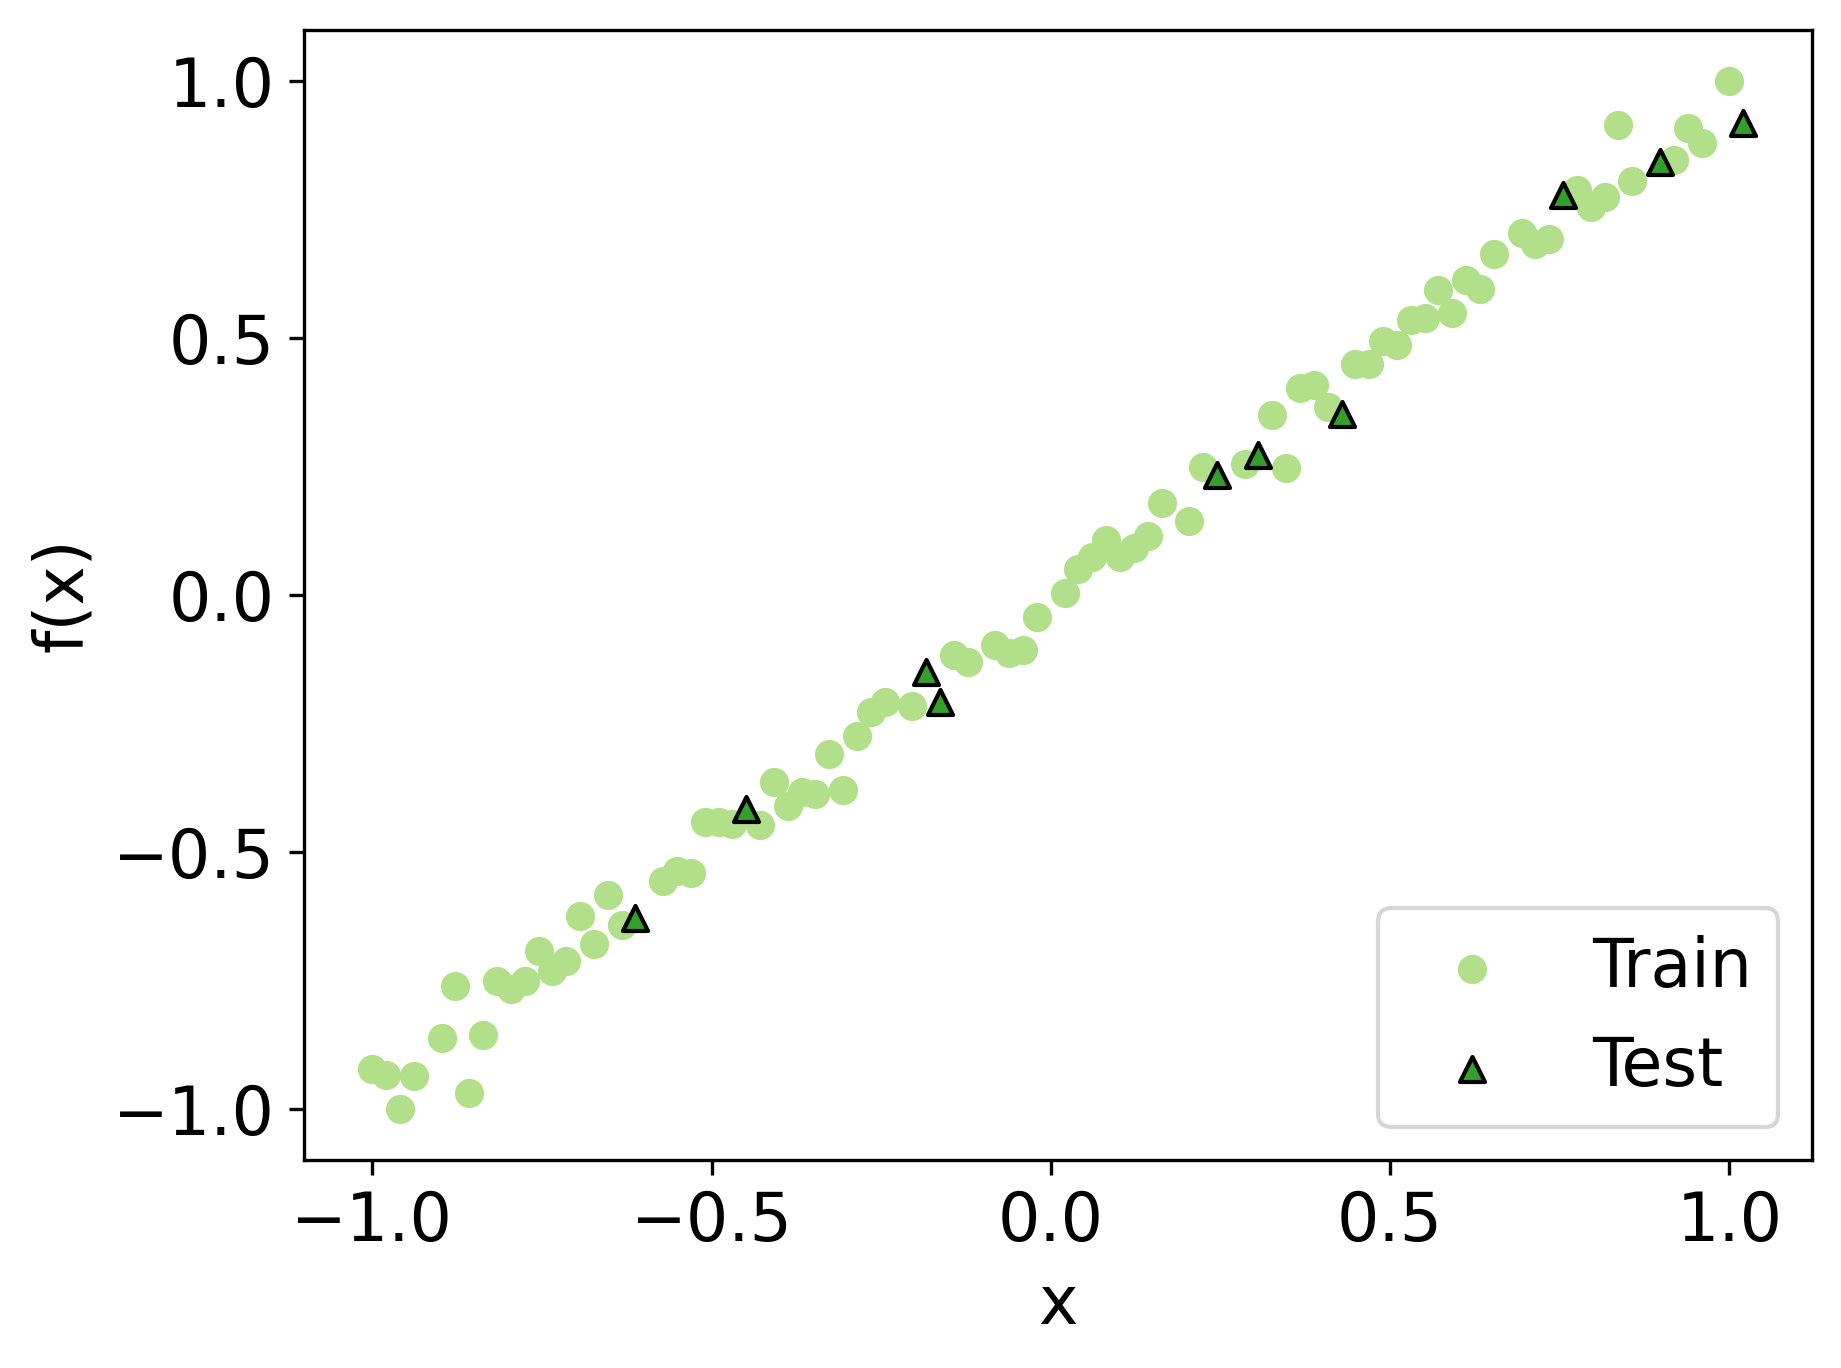
\includegraphics[width=\textwidth]{images/Function_Fitting/function_dataset/linear_train_vs_test.png}
		\caption{}
		\label{fig:linear_train_vs_test}
	\end{subfigure}
	\hfill
	\begin{subfigure}[b]{0.3\textwidth}
		\centering
		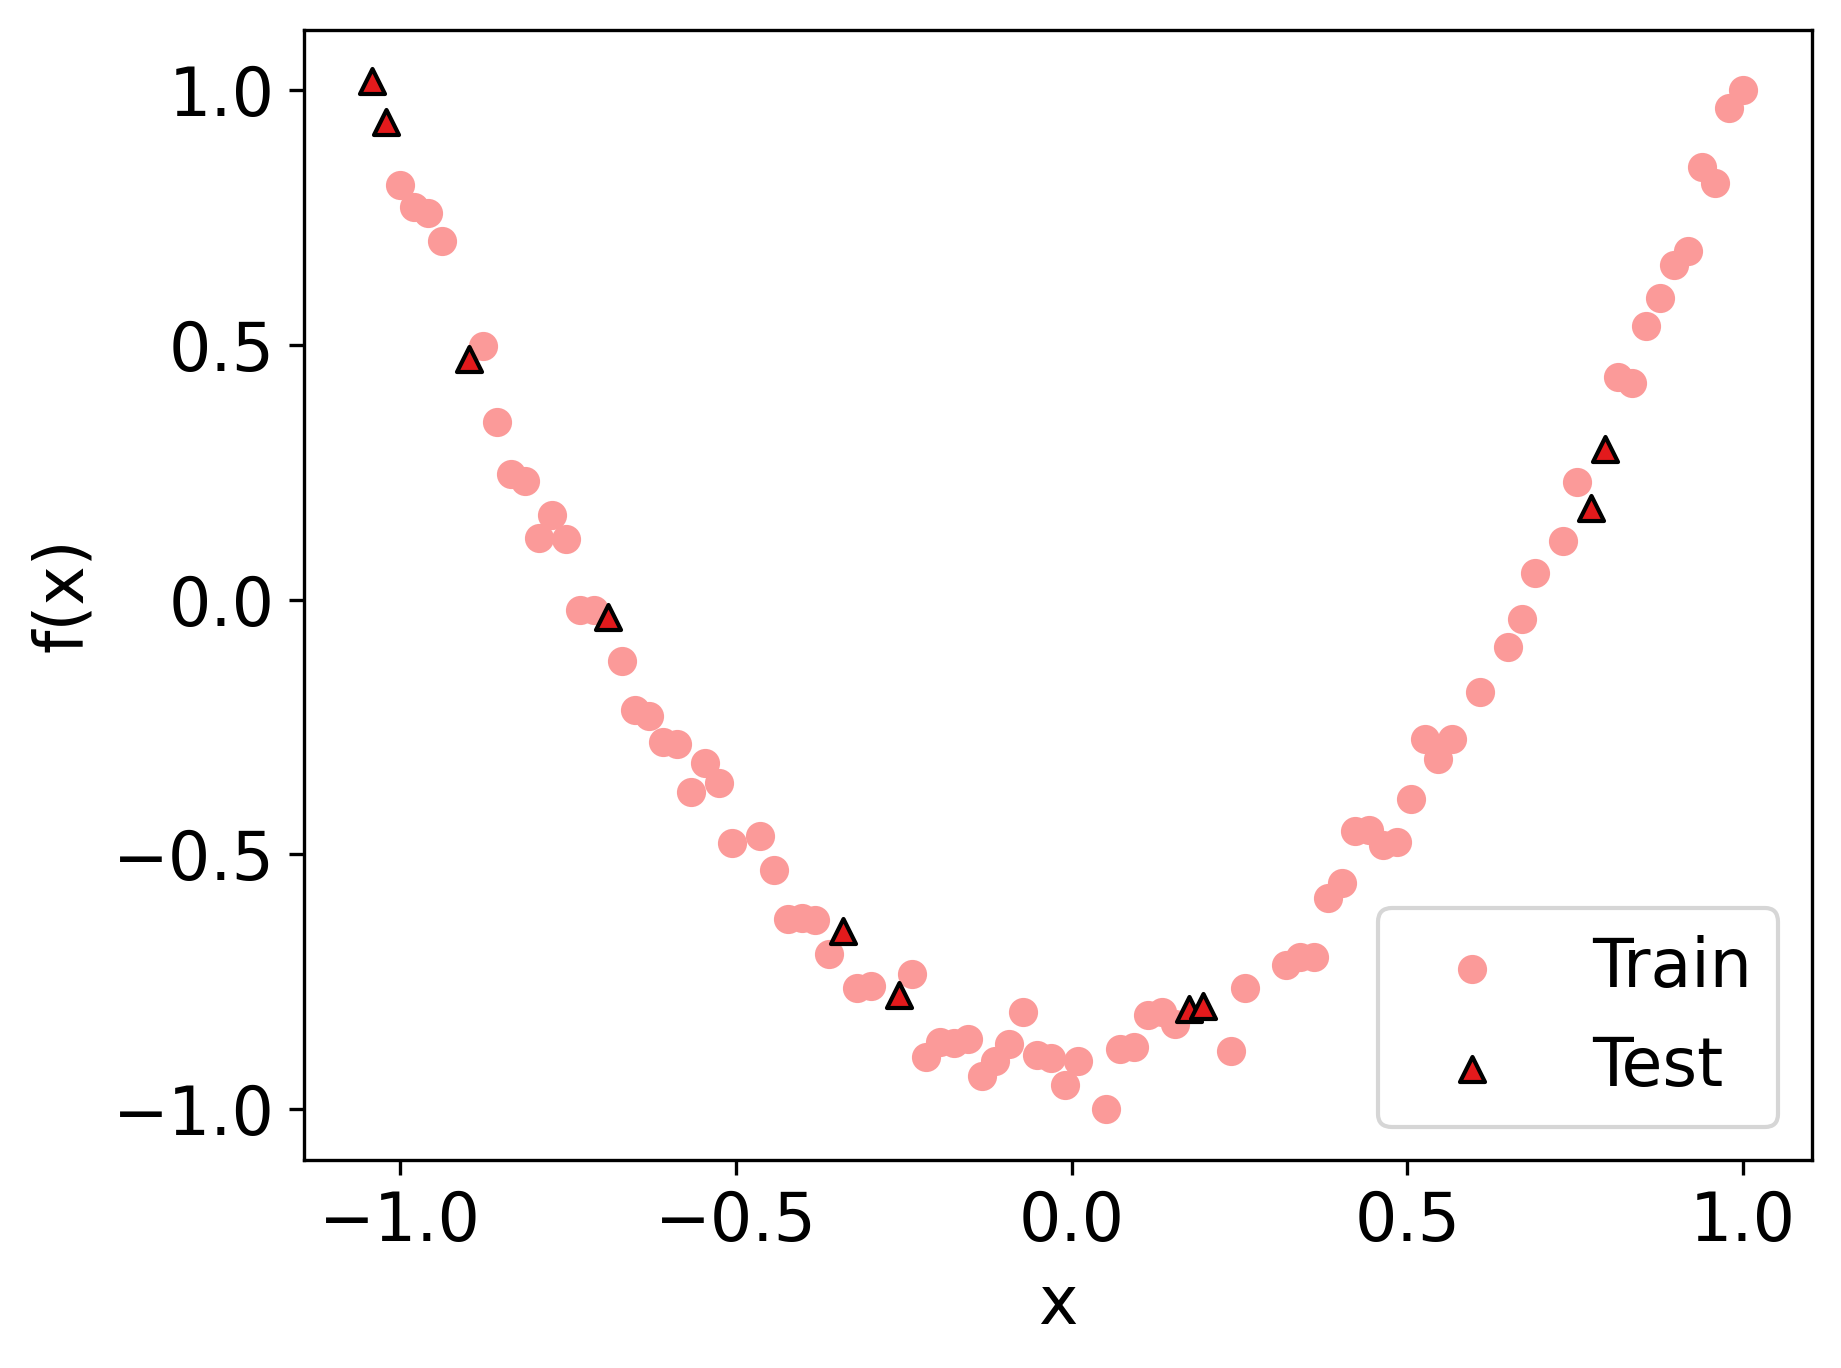
\includegraphics[width=\textwidth]{images/Function_Fitting/function_dataset/quadratic_train_vs_test.png}
		\caption{}
		\label{fig:quadratic_train_vs_test}
	\end{subfigure}
	\hfill
	\begin{subfigure}[b]{0.3\textwidth}
		\centering
		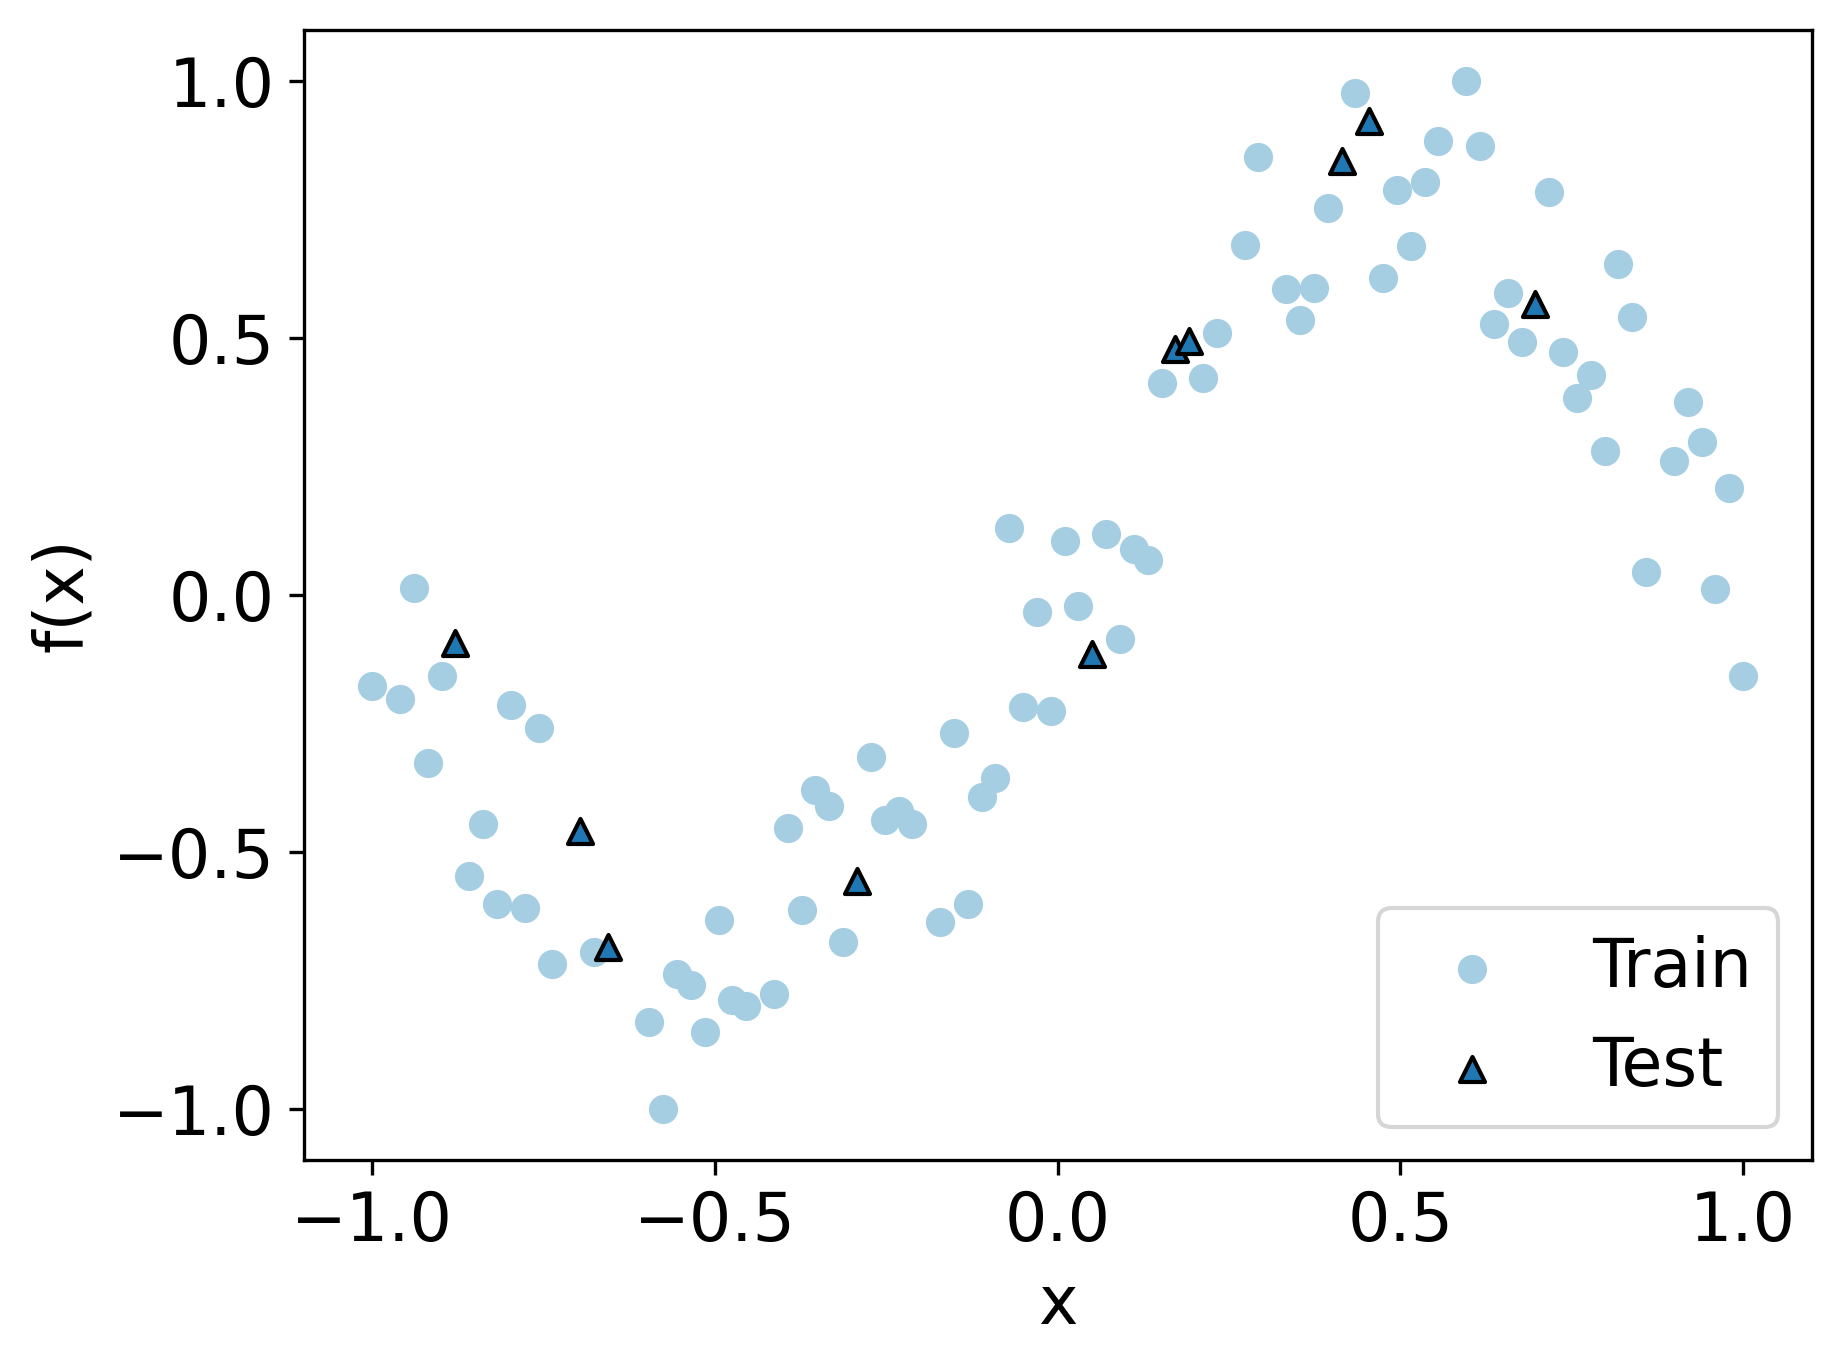
\includegraphics[width=\textwidth]{images/Function_Fitting/function_dataset/sine_train_vs_test.png}
		\caption{}
		\label{fig:sine_train_vs_test}
	\end{subfigure}
	\caption{}
	\label{fig:train_vs_test}
\end{figure}

\section{Results}
\subsection{Model Calibration Using Function fitting} 
We used the function fitting to determine if our models were implemented correctly.


\subsubsection{All (5 + 16 qubit)}
Figure \ref{fig:5qubit_Func_funcfit_R2} shows every encoder and ansatz pair explored for the function fitting datasest with 5 qubits.
\begin{figure}[H]
	\centering
	\begin{subfigure}[b]{\textwidth}
		\centering
		\includegraphics[width=\textwidth]{images/Function_Fitting/5qubit_Linear_funcfit_R2.png}
		\caption{}
		\label{fig:5qubit_Linear_funcfit_R2}
	\end{subfigure}
	\hfill
	\begin{subfigure}[b]{\textwidth}
		\centering
		\includegraphics[width=\textwidth]{images/Function_Fitting/5qubit_Quadratic_funcfit_R2.png}
		\caption{}
		\label{fig:5qubit_Quadratic_funcfit_R2}
	\end{subfigure}
	\hfill
	\begin{subfigure}[b]{\textwidth}
		\centering
		\includegraphics[width=\textwidth]{images/Function_Fitting/5qubit_Sine_funcfit_R2.png}
		\caption{}
		\label{fig:5qubit_Sine_funcfit_R2}
	\end{subfigure}
	\caption{}
	\label{fig:5qubit_Func_funcfit_R2}
\end{figure}


Figure \ref{fig:16qubit_Func_funcfit_R2} shows every encoder and ansatz pair explored for the function fitting datasest with 16 qubits.


\begin{figure}[H]
	\centering
	\begin{subfigure}[b]{\textwidth}
		\centering
		\includegraphics[width=\textwidth]{images/Function_Fitting/16qubit_Linear_funcfit_R2.png}
		\caption{}
		\label{fig:16qubit_Linear_funcfit_R2}
	\end{subfigure}
	\hfill
	\begin{subfigure}[b]{\textwidth}
		\centering
		\includegraphics[width=\textwidth]{images/Function_Fitting/16qubit_Quadratic_funcfit_R2.png}
		\caption{}
		\label{fig:16qubit_Quadratic_funcfit_R2}
	\end{subfigure}
	\hfill
	\begin{subfigure}[b]{\textwidth}
		\centering
		\includegraphics[width=\textwidth]{images/Function_Fitting/16qubit_Sine_funcfit_R2.png}
		\caption{}
		\label{fig:16qubit_Sine_funcfit_R2}
	\end{subfigure}
	\caption{}
	\label{fig:16qubit_Func_funcfit_R2}
\end{figure}



\subsubsection{RUD + AL (5 + 16 qubit)}\label{subsection:func_depth}
The best, median, and worst 5 were chosen from the 16 qubit data.

\begin{figure}[H]
	\centering
	\begin{subfigure}[b]{\textwidth}
		\centering
		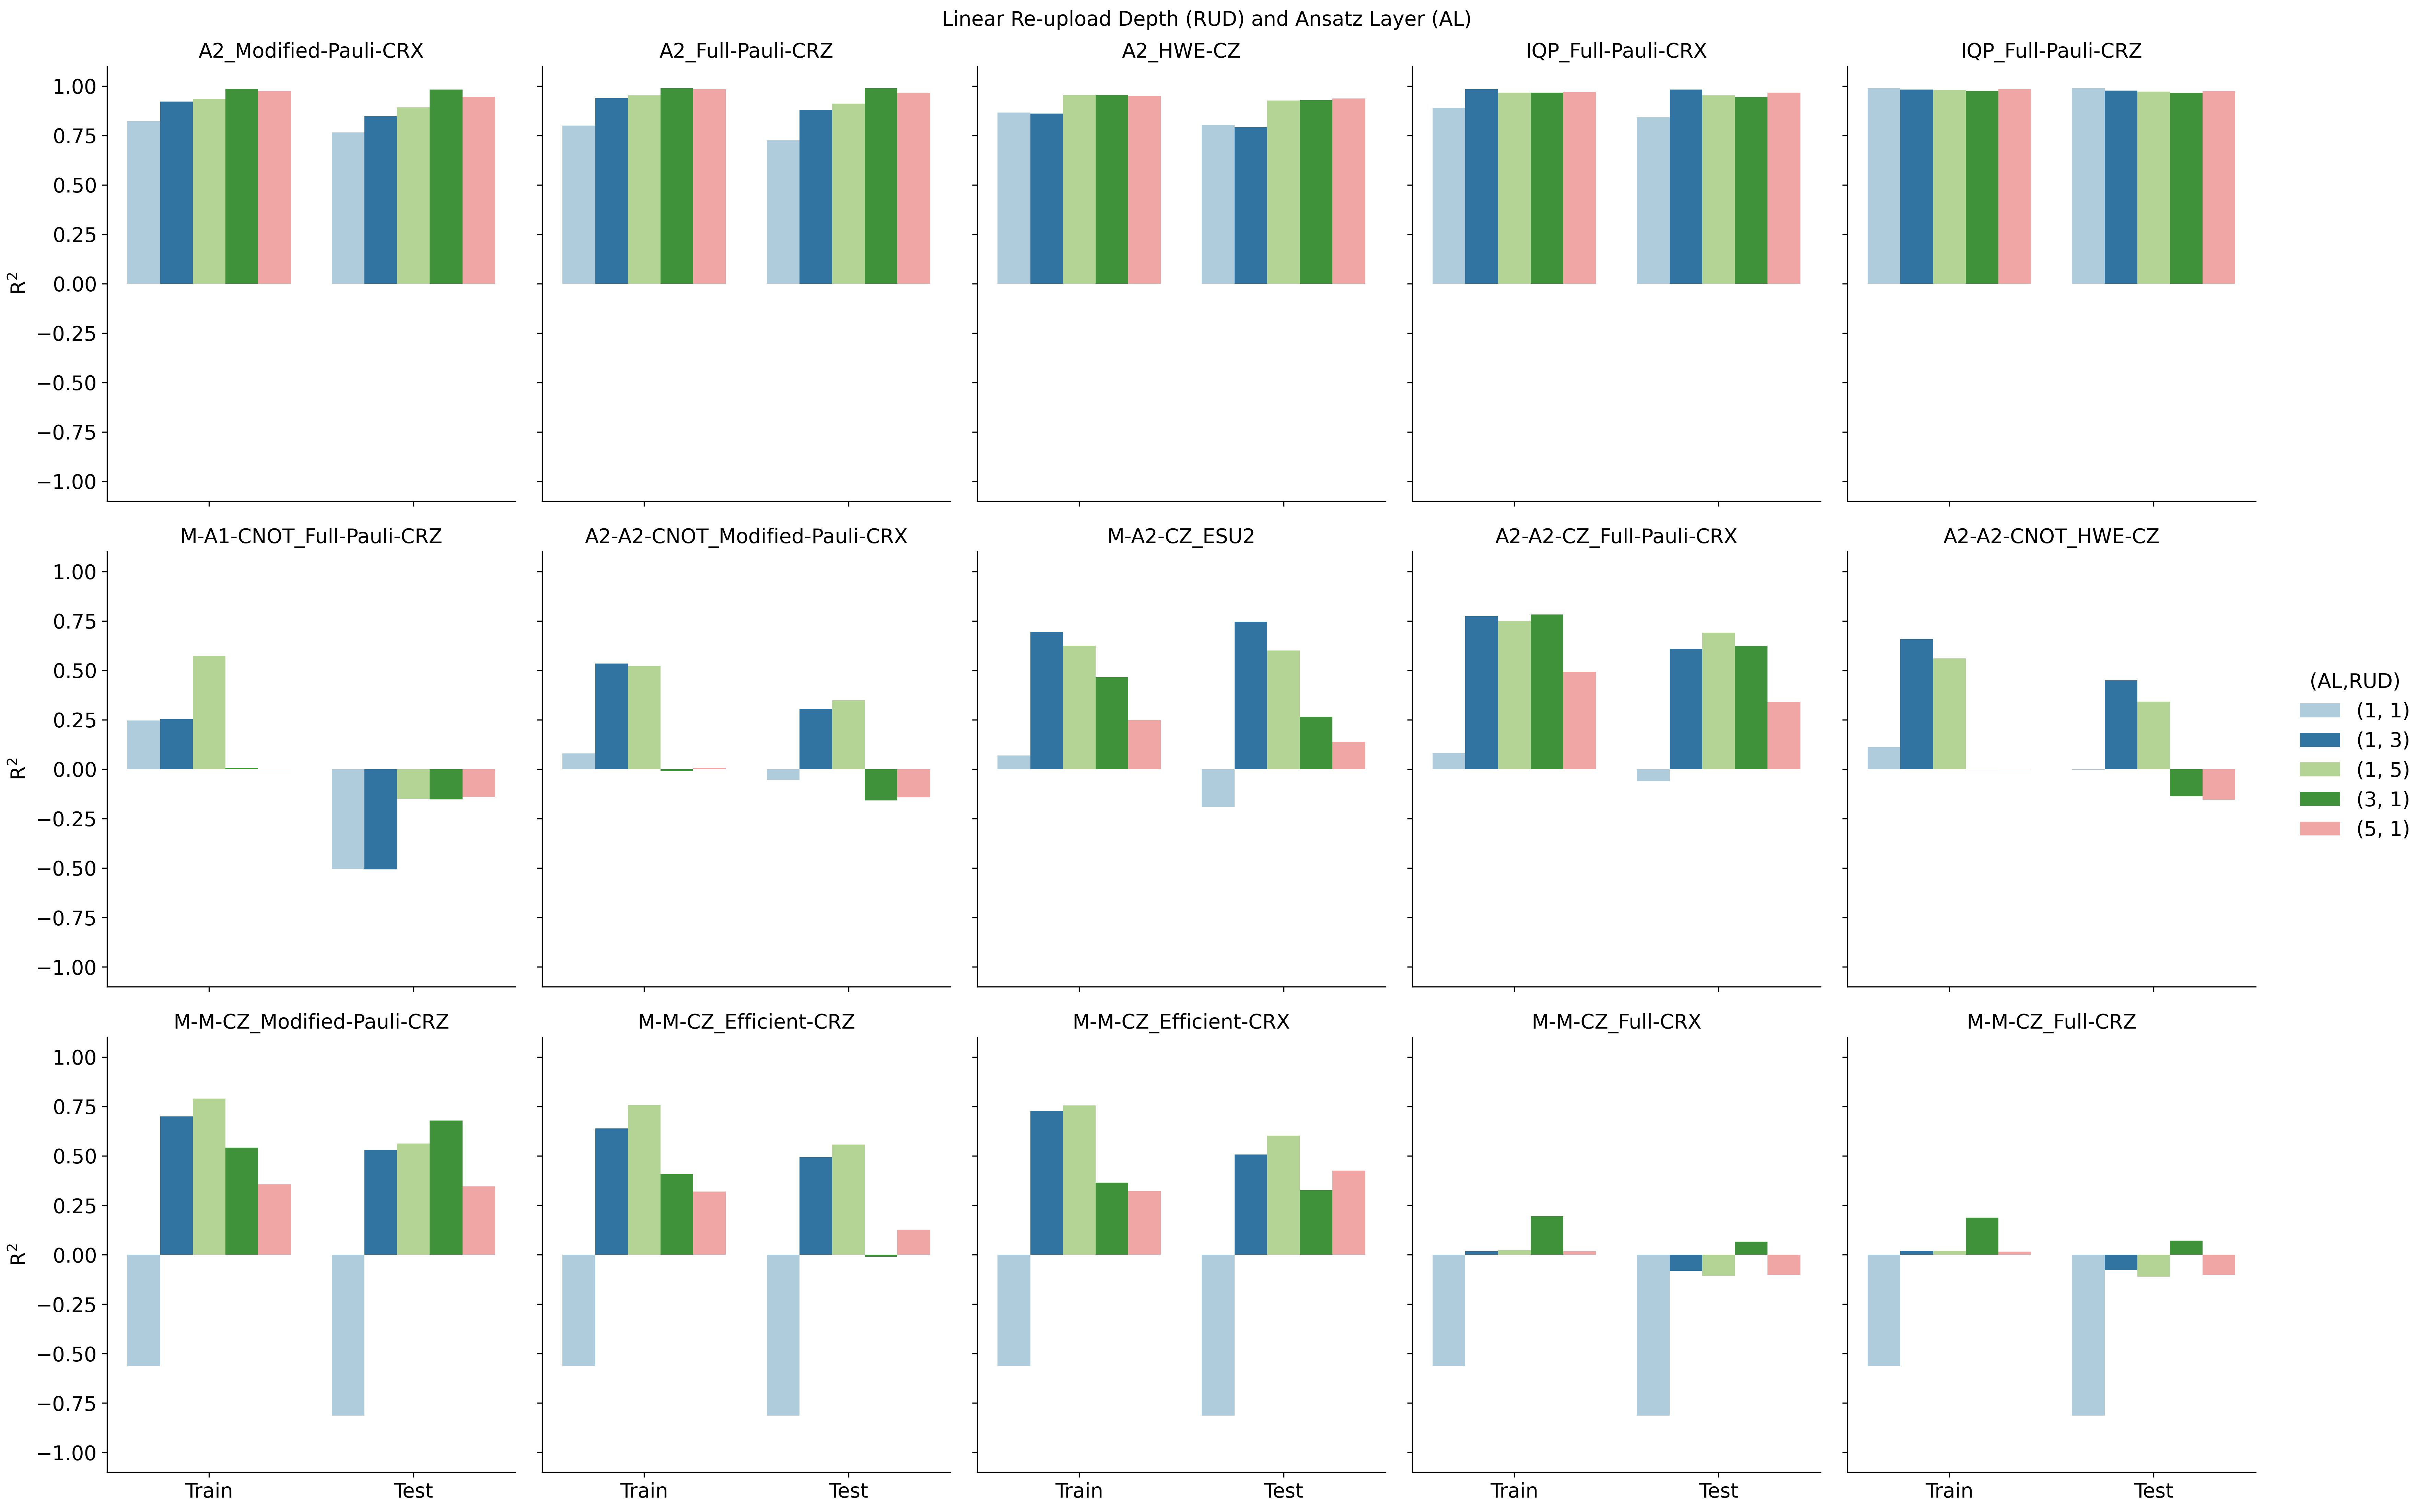
\includegraphics[width=\textwidth]{images/Function_Fitting/16qubit_Linear_RUD_AL.png}
		\caption{}
		\label{fig:16qubit_Linear_RUD_AL}
	\end{subfigure}
	\hfill
	\begin{subfigure}[b]{\textwidth}
		\centering
		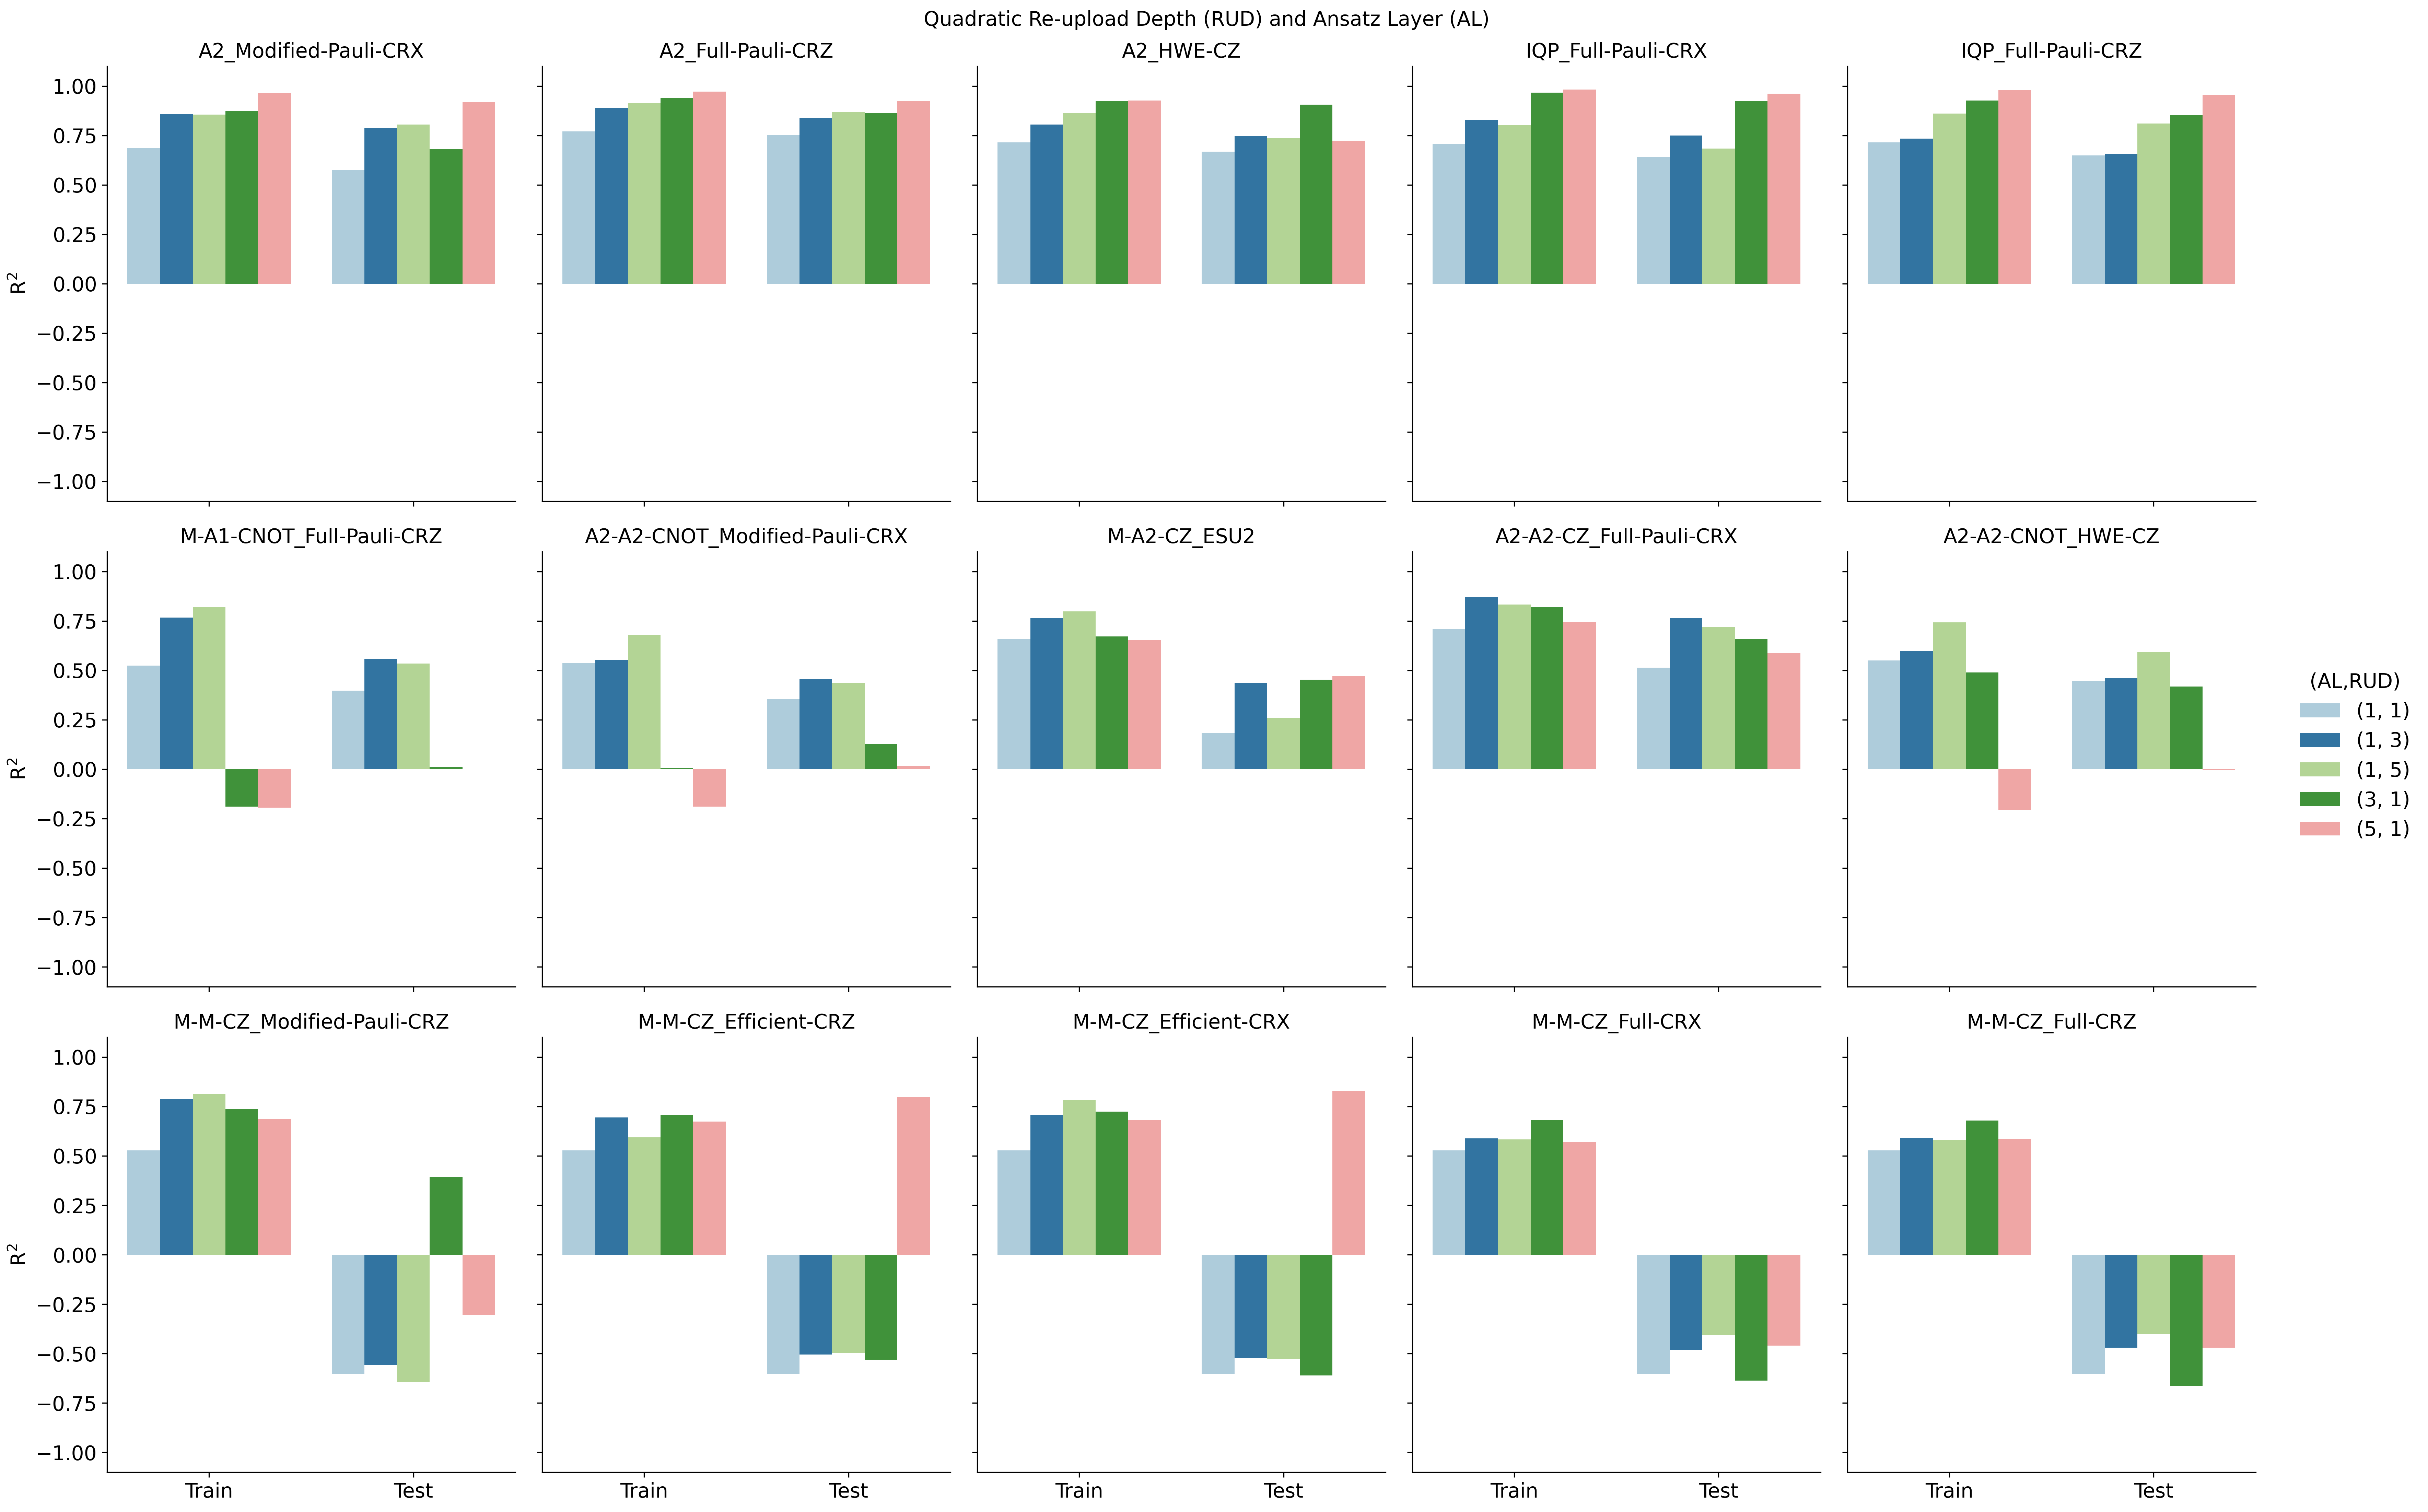
\includegraphics[width=\textwidth]{images/Function_Fitting/16qubit_Quadratic_RUD_AL.png}
		\caption{}
		\label{fig:16qubit_Quadratic_RUD_AL}
	\end{subfigure}
	\hfill
	\begin{subfigure}[b]{\textwidth}
		\centering
		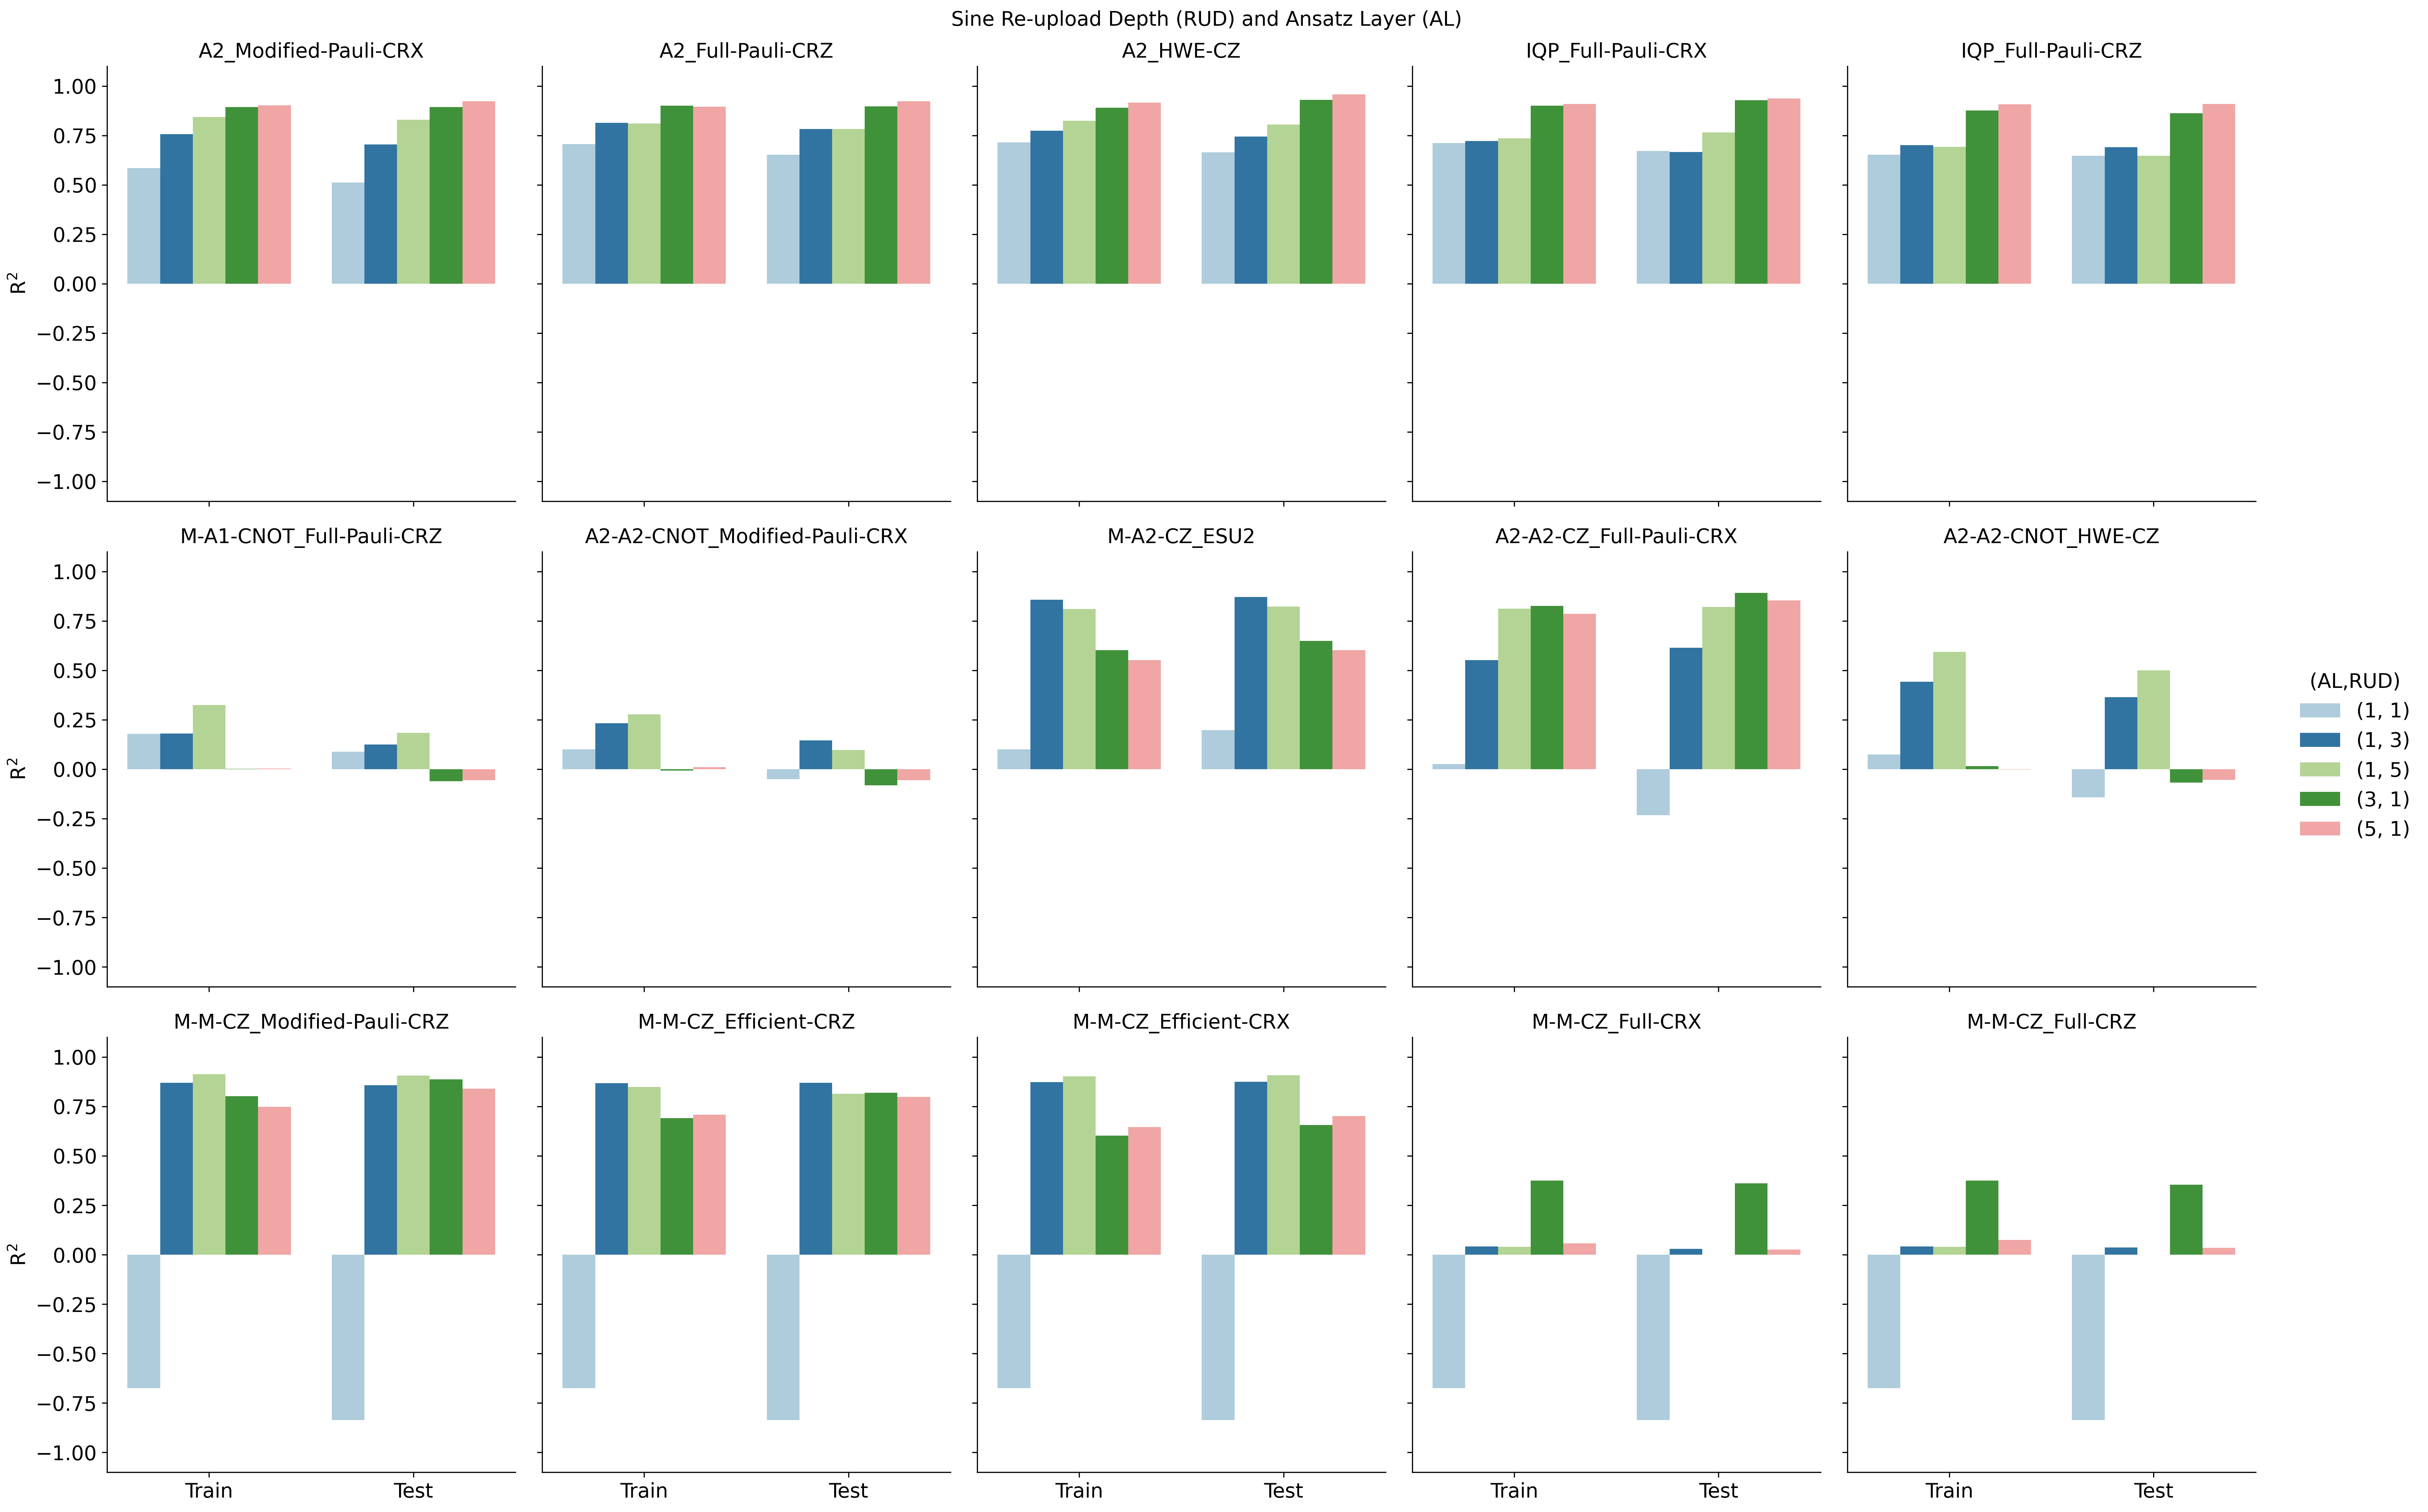
\includegraphics[width=\textwidth]{images/Function_Fitting/16qubit_Sine_RUD_AL.png}
		\caption{}
		\label{fig:16qubit_Sine_RUD_AL}
	\end{subfigure}
	\caption{}
	\label{fig:16qubit_Func_RUD_AL}
\end{figure}

\subsubsection{Learning curve}
The best models from Section \ref{subsection:func_depth} were then used to compare them with classical machine learning models using learning curves, where the test set was held to 10 points, while the training data was varied from 10-80 points.

For the linear model with 16 qubits, the IQP encoding with the Full Pauli CRZ ansatz layer outperforms the classical models at 10\% of the training data, as show in  Fig. \ref{fig:linear_learning_curves}.
The quantum model is less overfit and has a more accurate test score than any of the classical models. 
As the training set size increases, the quantum model maintains an average train and test R$^{2}$ of 0.98, while the classical models maintain an average train and test R$^{2}$ of 0.99.
\begin{figure}[H]
	\centering
	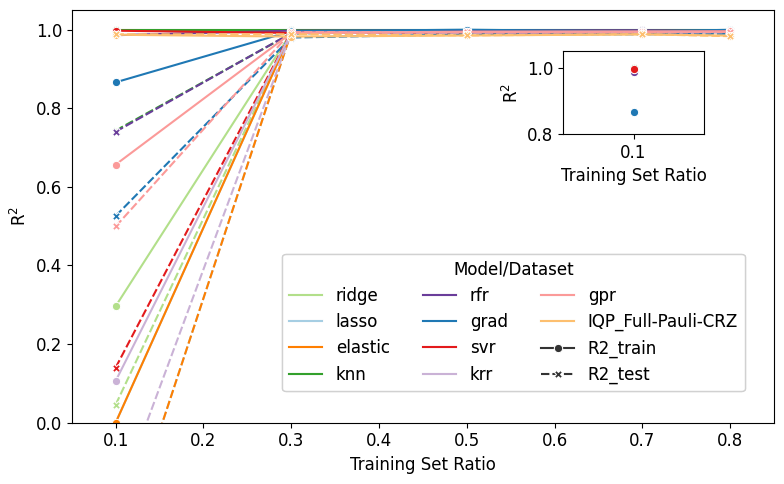
\includegraphics[width=\textwidth]{images/Function_Fitting/linear_learning_curves.png}
	\caption{Linear learning curve}
	\label{fig:linear_learning_curves}
\end{figure}

A2 HWE-CZ
Performs better than all but 
\begin{figure}[H]
	\centering
	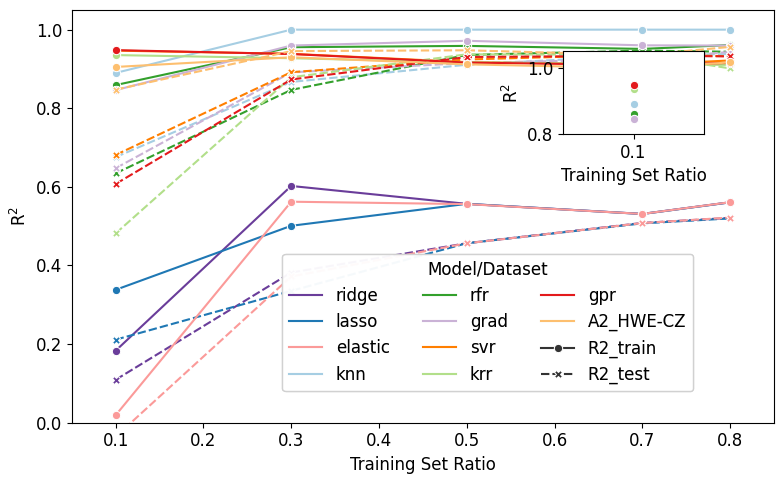
\includegraphics[width=\textwidth]{images/Function_Fitting/sine_learning_curves.png}
	\caption{sine learning curve}
	\label{fig:sine_learning_curves}
\end{figure}


\subsubsection{Error mitigation}
FakeQuebec backend
ZNE linear and Richardson
TREX
Without

\subsubsection{Real device}
IBM Quebec!

\subsection{BSE} 

\subsubsection{Classical testing}
After an extensive search of the possible moleuclar representations for the BSE dataset, we decided to use Morgan fingerprints.
To map this set of features down to 5 and 16 qubits, we analyzed using SHapley Additive exPlanation (SHAP) values and principal component analysis.
Based of of the analysis from Fig. \ref{fig:Feat_redR2}, we chose to use the set of features reduced using PCA due to the more accurate, albiet overfit data.
\begin{figure}[H]
	\centering
	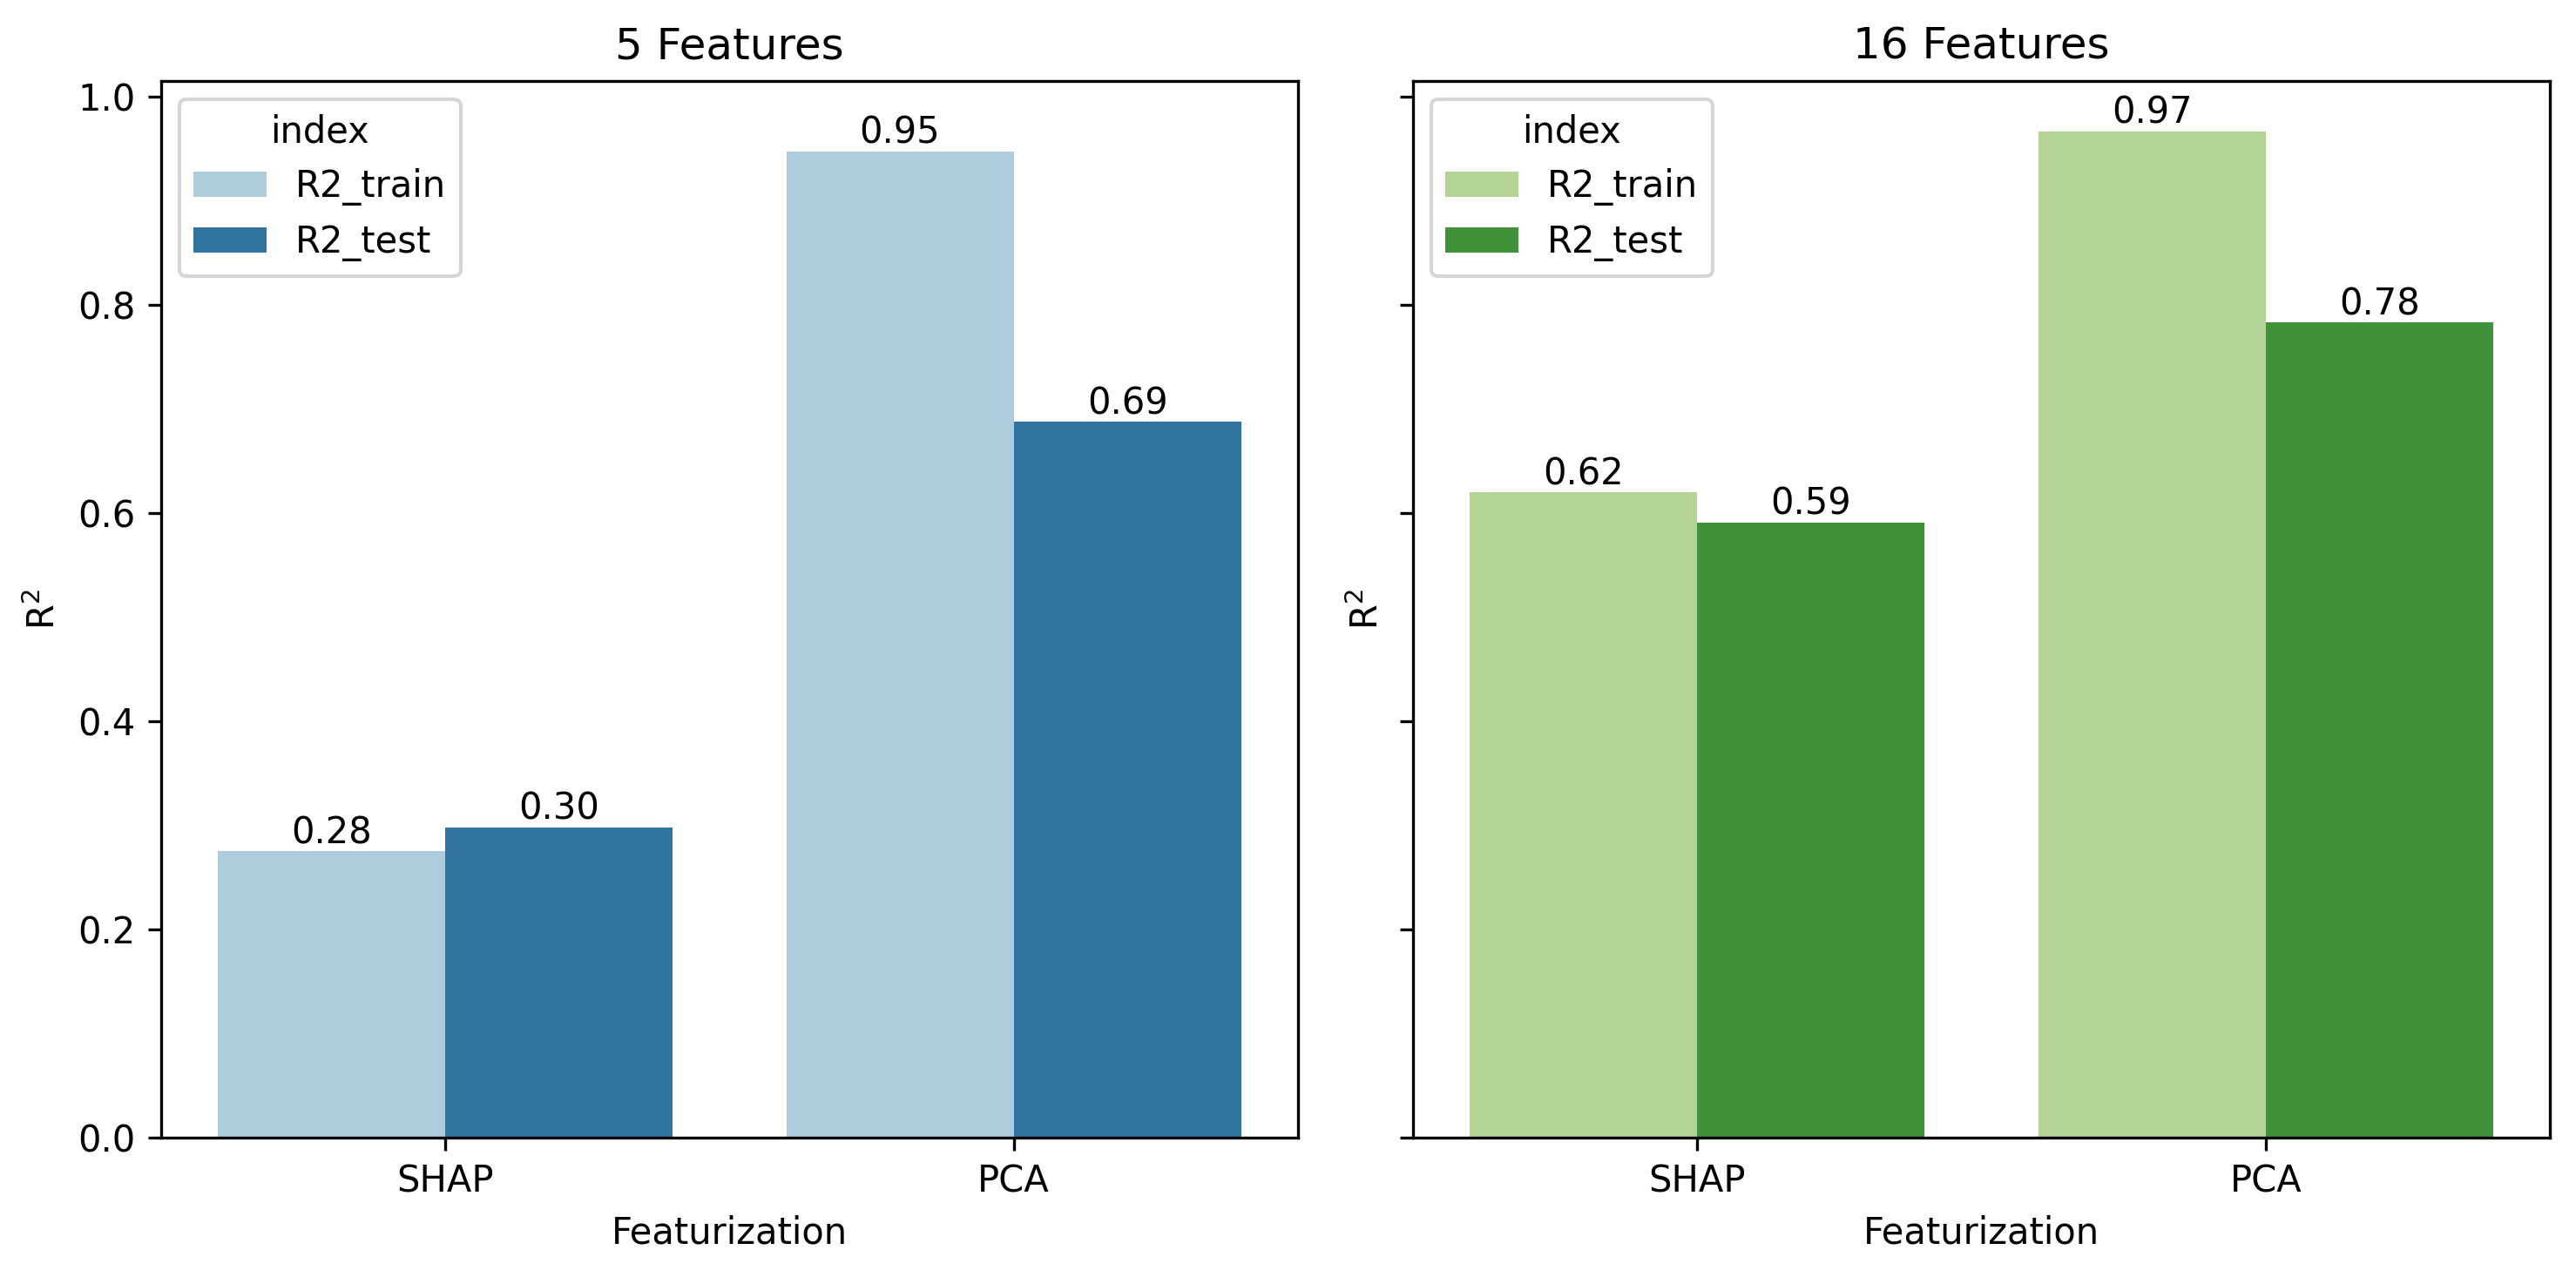
\includegraphics[width=\textwidth]{images/BSE/Feat_redR2.png}
	\caption{BSE Feature Reduction}
	\label{fig:Feat_redR2}
\end{figure}
\subsubsection{All (5 + 16 qubit)}
Using the aforementioned datasets, along with the 168 encoder-ansatz pairs we analyzed the cost of modeling the BSE dataset using the 5 qubit feature set first.

\begin{figure}[H]
	\centering
	\includegraphics[width=\textwidth]{images/BSE/5qubit_BSE_MAE.png}
	\caption{5 qubit BSE MAE (kcal/mol)}
	\label{fig:5qubit_BSE_MAE}
\end{figure}



\begin{figure}[H]
	\centering
	\includegraphics[width=\textwidth]{images/BSE/16qubit_BSE_MAE.png}
	\caption{16 qubit BSE MAE (kcal/mol)}
	\label{fig:16qubit_BSE_MAE}
\end{figure}

Using this data, we analyzed the mean time per training iteration versus the MAE and circuit depth. 
We found that within the 168 encoder-ansatz pairs, there existed a bimodal distribution, where there were a set of 70 circuits with the mean time per iteration greater than 100 seconds and those with less.
Going forward, we will only use the set of circuits that belong to the set with mean iteration times less than 100 seconds due to cost considerations.
\begin{figure}[H]
	\centering
	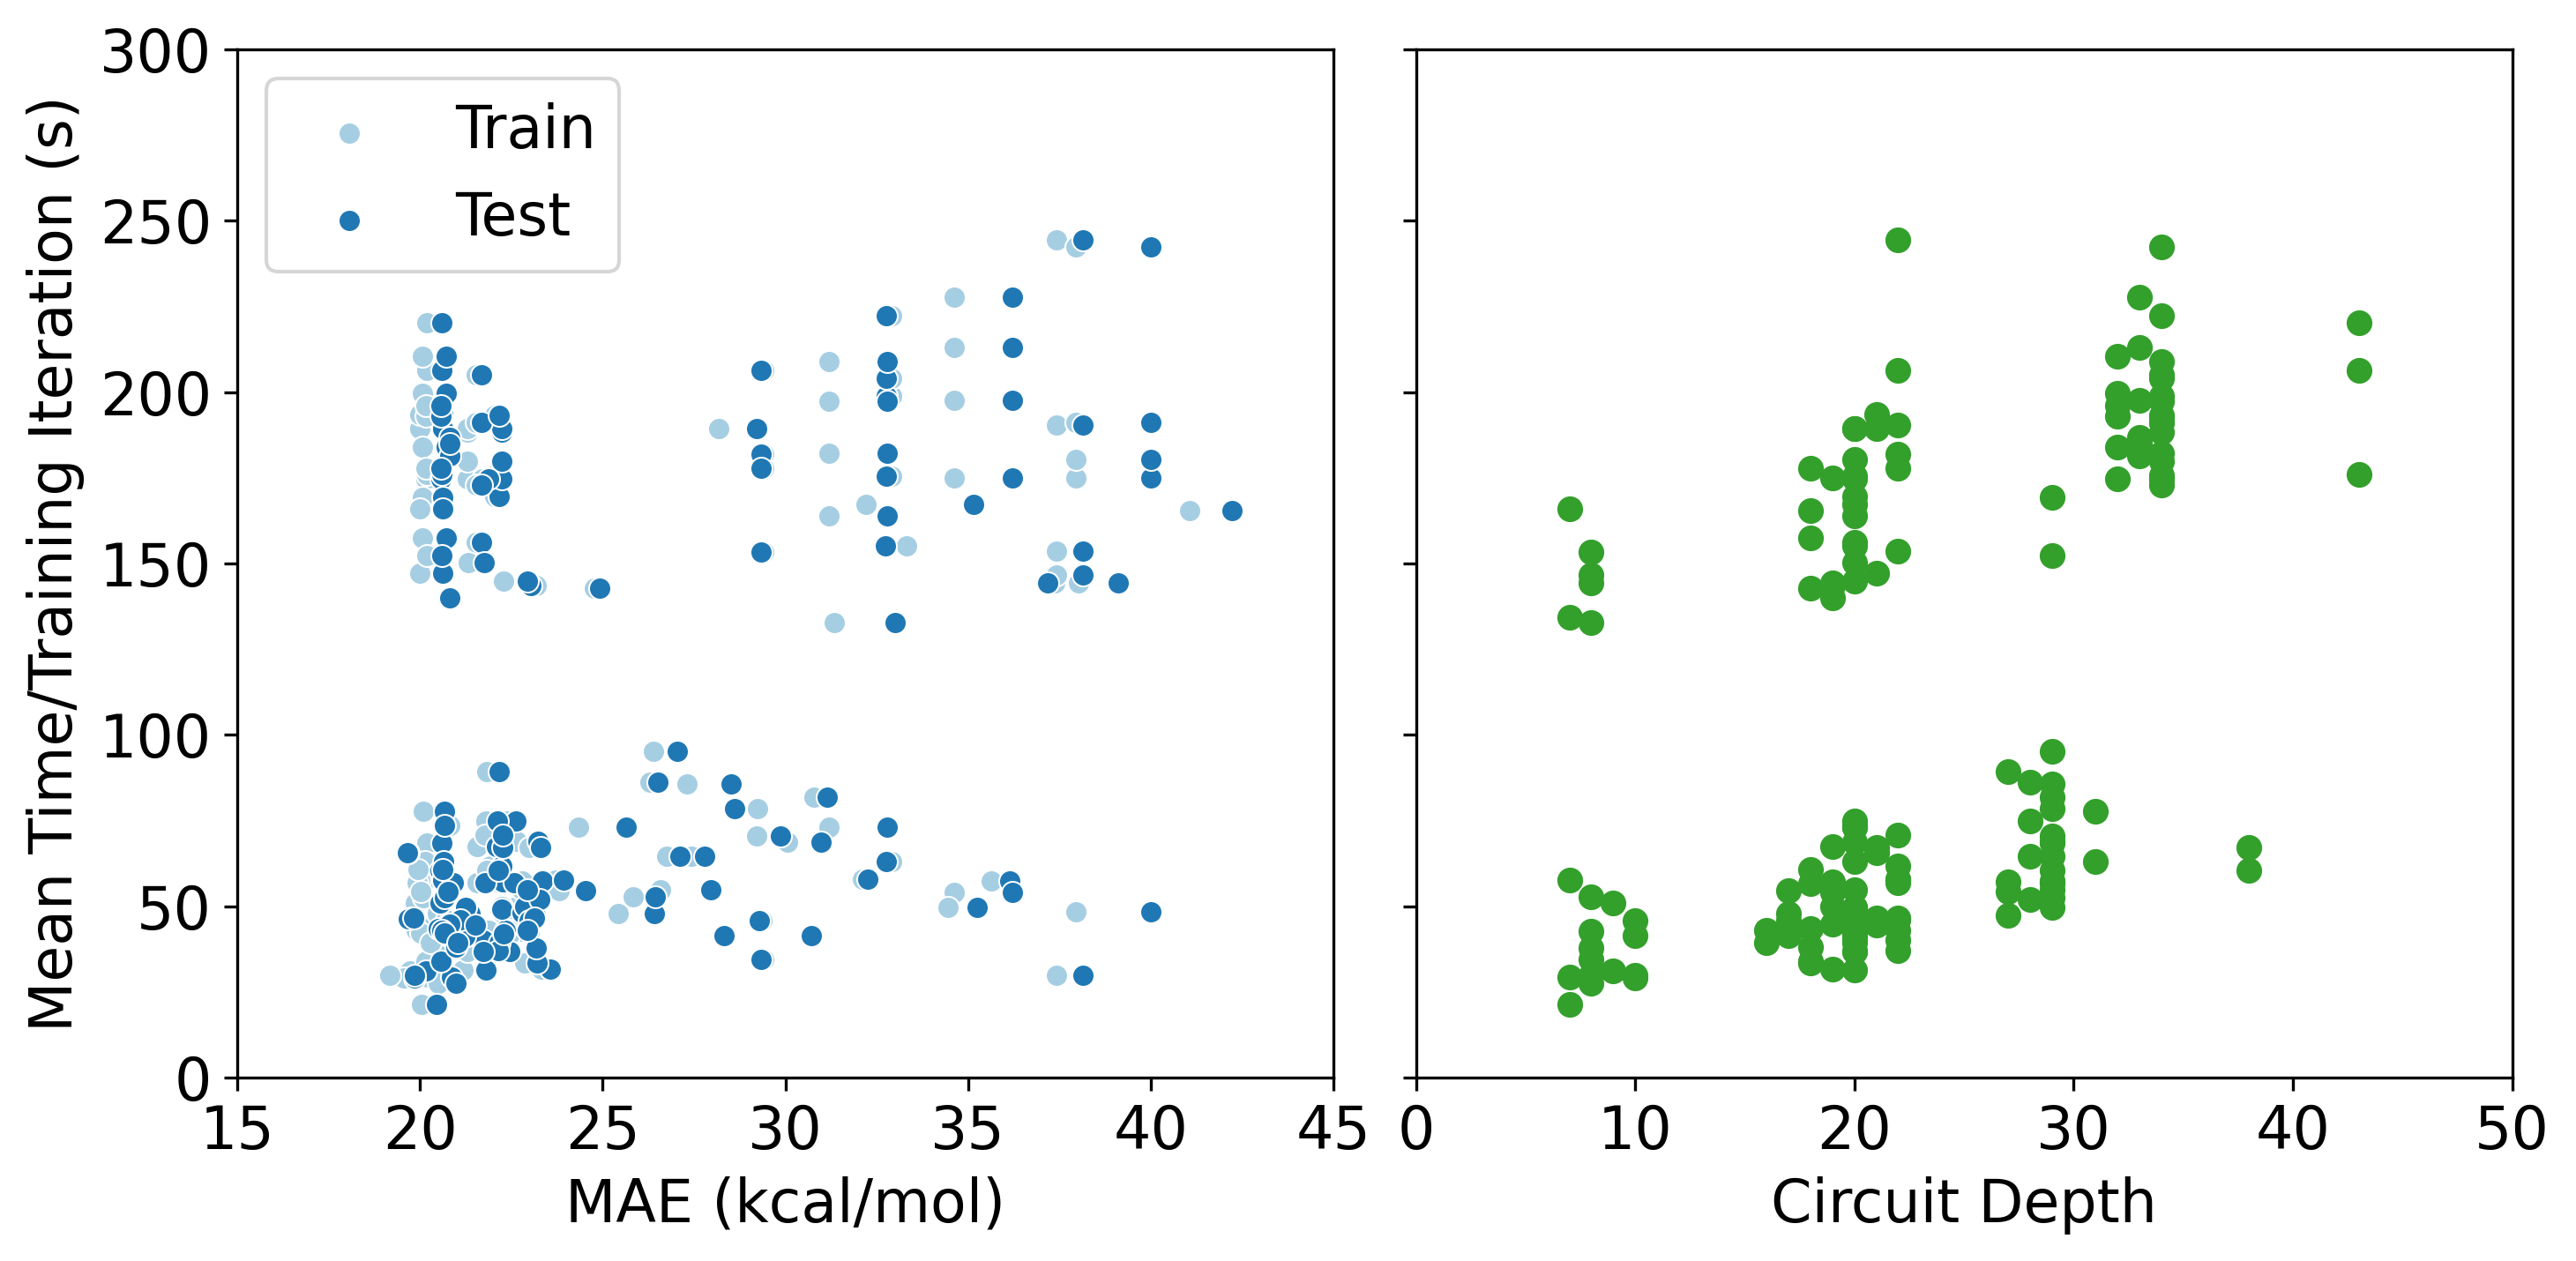
\includegraphics[width=\textwidth]{images/BSE/AllBSE5_circuitdepth_MAE_vs_iterationtime.png}
	\caption{5 qubit BSE MAE (kcal/mol)}
	\label{fig:AllBSE5_circuitdepth_MAE_vs_iterationtime}
\end{figure}

For the 70 circuits that belong to those with iterations less than 100 seconds for the BSE 5 qubit set, we used these for the 16 qubit as well and found that...



\subsubsection{RUD + AL (5 + 16 qubit)}
Based off of the improvements shown in the function fitting dataset, we only used the best encoding ansatz pair for the real datasets
For the 5 qubit, it is  M-M-CZ HWE-CNOT

\begin{figure}[H]
	\centering
	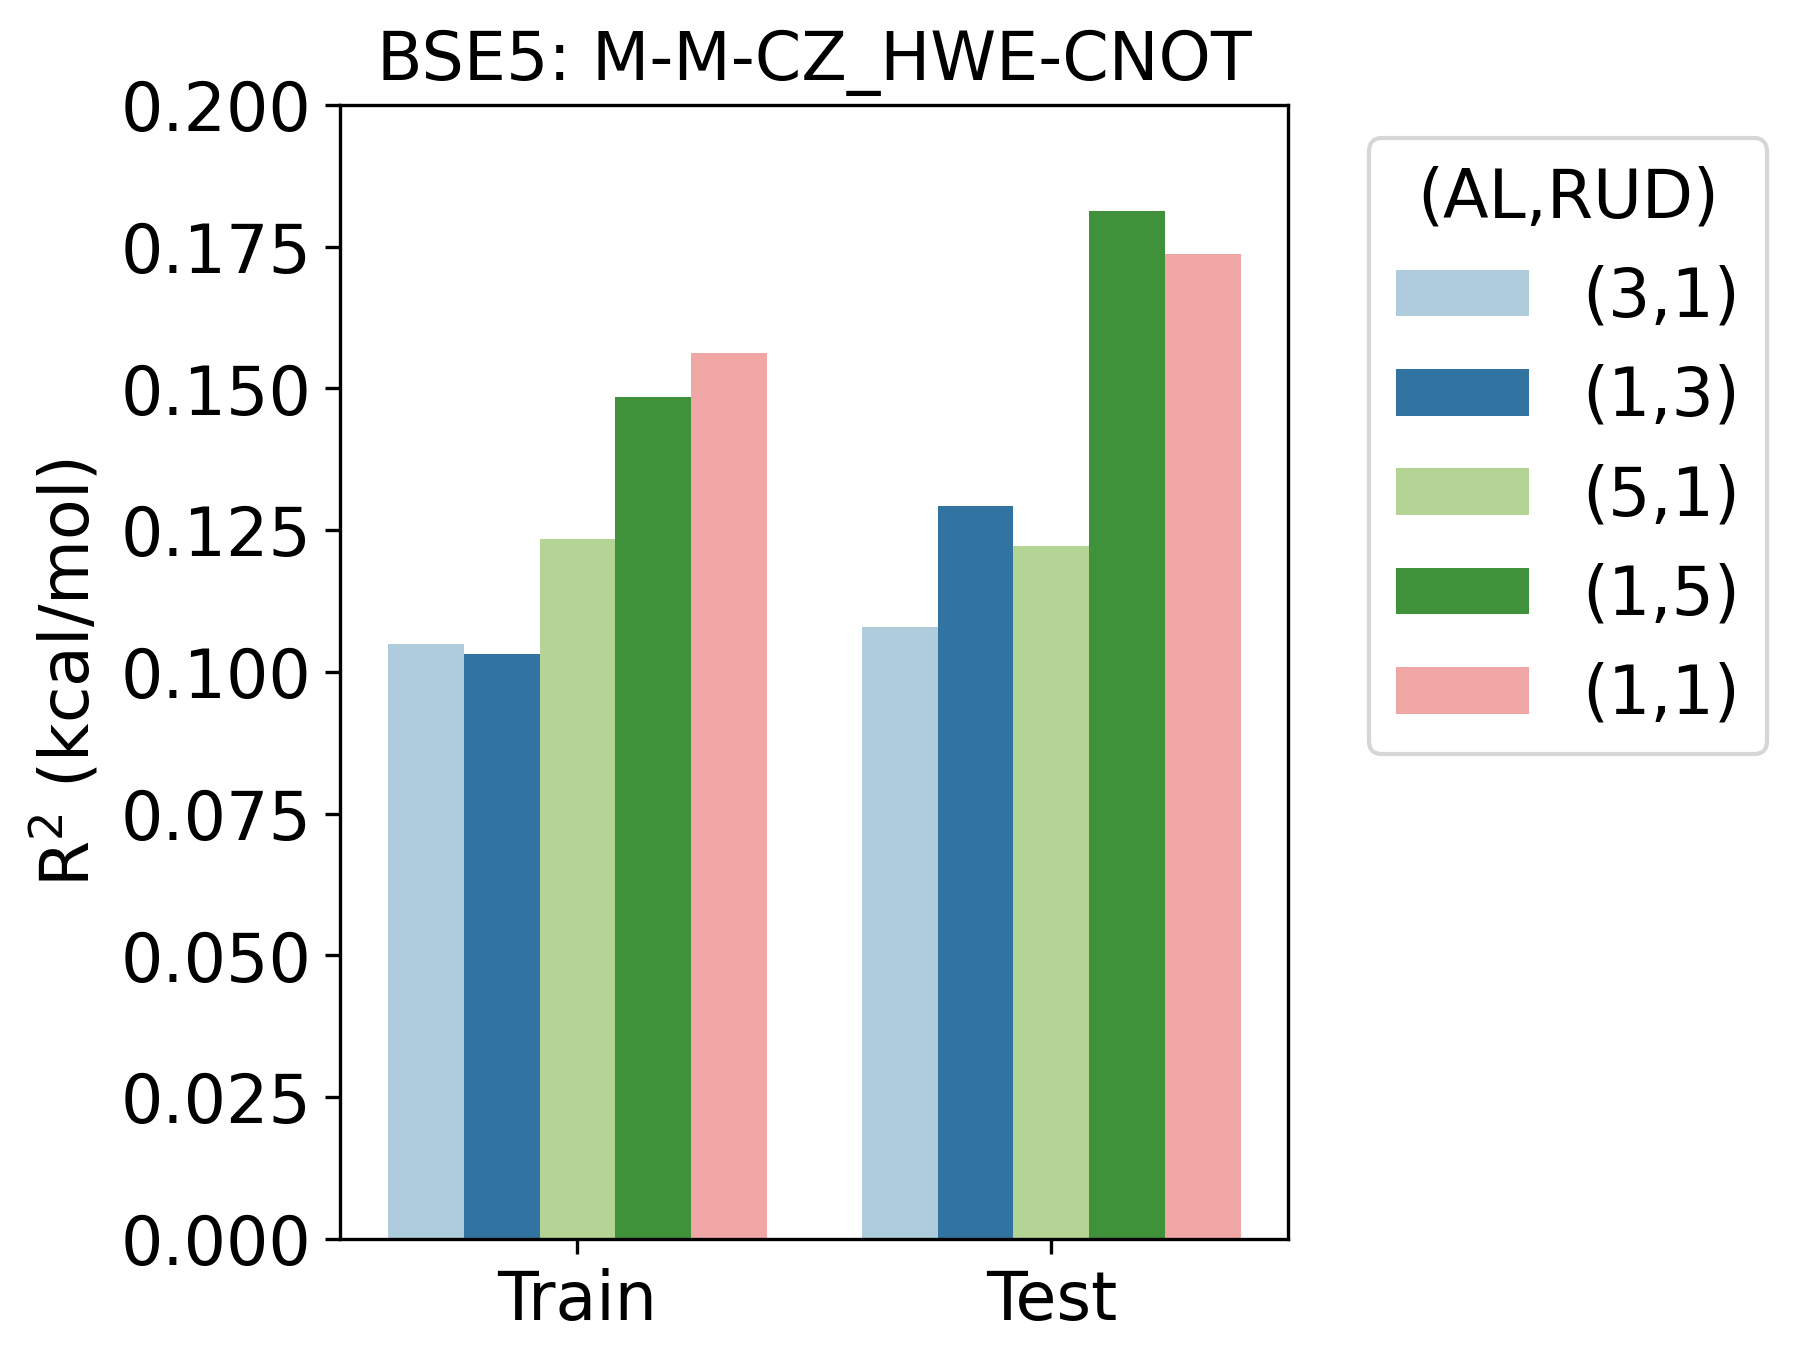
\includegraphics[width=\textwidth]{images/BSE/BSE5_RUDAL.png}
	\caption{5 qubit BSE MAE (kcal/mol) AL RUD}
	\label{fig:	BSE5_RUDAL}
\end{figure}

For 16 qubit A2 Hadamard


\subsubsection{Error mitigation}
\subsubsection{Real device}

\subsection{DDCC} 

\subsubsection{Classical testing}
\subsubsection{All (5 + 16 qubit)}
\subsubsection{RUD + AL (5 + 16 qubit)}
\subsubsection{Error mitigation}
\subsubsection{Real device}

\section{Conclusion}
Depth is not always better!
Molecular representations specifically for QML
Distributed QC to incorporate more features

\bibliography{achemso-demo}

\end{document}
